% ======================================================================
% Scientific Reports — Article. Build this file.
% main_CM.tex (Communications Medicine) and main.tex (npj Digital
% Medicine) remain buildable and unchanged.
%
% Journal format (https://www.nature.com/srep/author-instructions/
% submission-guidelines):
%   title            <= 20 words, one scientifically accurate sentence
%   abstract         <= 200 words, unstructured, unreferenced
%   keywords         <= 6
%   section order    Introduction, Results (subheadings), Discussion
%                    (no subheadings), Methods
%   main text        <= 4,500 words (abstract, Methods, references and
%                    legends not counted)
%   display items    <= 8 figures and tables, each table <= one page
%   references       ~60, numeric, square brackets, Nature style
%   Data availability statement before the References
%   Supplementary Information as a single separate PDF whose first page
%   carries the title and author list; items numbered S1, S2, ...
% Verify with: python wordcount_sr.py
%
% Peer review: Scientific Reports is single-anonymised by default. Set
% \anontrue below to produce the double-anonymised variant (no authors,
% affiliations, acknowledgements, contributions, funding or identifying
% URLs) if that option is selected in the submission system.
%
% Build (article + supplement, cross-referenced):  .\build_SR.ps1
% ======================================================================
\documentclass[12pt,a4paper]{article}

\newif\ifanon
\anonfalse

\newcommand{\SRexternaldoc}{supplementary_SR}
\newcommand{\SRpdftitle}{A translatability verdict for cross-domain medical prediction that reports what a scarce cohort can adjudicate}
\newcommand{\SRrunninghead}{A translatability verdict for cross-domain medical prediction}
% ============================================================
% Preamble — Scientific Reports build (main_SR.tex and
% supplementary_SR.tex share it).
% Journal guidance (https://www.nature.com/srep/author-instructions/
% submission-guidelines): single-column, unjustified text; Arabic page
% number in the footer; default Computer Modern fonts; numeric citations
% in square brackets in Nature style; line numbers recommended;
% equations cited as "equation (1)".
%
% The file that \input{}s this preamble must define \SRexternaldoc
% (the jobname of the companion document whose labels are read with
% xr-hyper: the article reads the supplement and vice versa) and
% \SRpdftitle.
% ============================================================

\usepackage[utf8]{inputenc}
\usepackage[T1]{fontenc}
\usepackage[english]{babel}
\usepackage{lmodern}
\usepackage{microtype}

\usepackage[a4paper,top=25mm,bottom=25mm,left=25mm,right=25mm]{geometry}
\usepackage{setspace}
\onehalfspacing
% Unjustified single-column text, as the journal asks of revised files.
\usepackage[document]{ragged2e}
\setlength{\RaggedRightParindent}{\parindent}

% Line numbers on every page of the article (journal recommendation).
\usepackage[mathlines]{lineno}
\linenumbers
\renewcommand\linenumberfont{\normalfont\tiny\color{gray}}

\usepackage{amsmath,amssymb,bm,mathtools}
\usepackage{graphicx}
\graphicspath{{figures/casegrid_1600/}{figures/}}
\usepackage{float}
\usepackage{placeins}
\usepackage{subcaption}
\usepackage[labelfont=bf,font=small]{caption}

\setcounter{topnumber}{3}
\setcounter{bottomnumber}{2}
\setcounter{totalnumber}{4}
\renewcommand{\topfraction}{0.9}
\renewcommand{\bottomfraction}{0.7}
\renewcommand{\textfraction}{0.1}
\renewcommand{\floatpagefraction}{0.5}

% Inside table floats the size ladder is the 10 pt one (normal 10,
% small 9, footnote 8, script 7) so that no table overruns one page.
\usepackage{etoolbox}
\newcommand{\tablesizes}{%
  \renewcommand{\normalsize}{\fontsize{10}{12}\selectfont}%
  \renewcommand{\small}{\fontsize{9}{10.5}\selectfont}%
  \renewcommand{\footnotesize}{\fontsize{8}{9.5}\selectfont}%
  \renewcommand{\scriptsize}{\fontsize{7}{8}\selectfont}%
  \normalsize}
% Inside floats the ragged2e paragraph indent is dropped, otherwise a
% \resizebox{\linewidth} table starts an indented paragraph and overruns
% the text block by exactly \parindent.
\AtBeginEnvironment{table}{\tablesizes\setlength{\parindent}{0pt}%
  \setlength{\RaggedRightParindent}{0pt}\setlength{\CenteringParindent}{0pt}}
\AtBeginEnvironment{figure}{\setlength{\parindent}{0pt}%
  \setlength{\RaggedRightParindent}{0pt}\setlength{\CenteringParindent}{0pt}}

\usepackage{booktabs,multirow,makecell,longtable,tabularx,array}
\newcolumntype{C}[1]{>{\centering\arraybackslash}p{#1}}
\newcolumntype{L}[1]{>{\raggedright\arraybackslash}p{#1}}

\usepackage[dvipsnames,table]{xcolor}
\definecolor{linkblue}{RGB}{0,70,140}

% Cross-document references: the article cites Supplementary items and
% the Supplementary Information cites main-text equations, tables and
% figures. xr-hyper must precede hyperref.
\usepackage{xr-hyper}
% [nocite]: import labels only, not the other document's \bibcite
% entries (each document carries its own numbered reference list).
\externaldocument[][nocite]{\SRexternaldoc}

\usepackage[colorlinks,linkcolor=linkblue,citecolor=linkblue,urlcolor=linkblue,
  pdftitle={\SRpdftitle}]{hyperref}
\usepackage{xurl}
\usepackage[capitalise,noabbrev]{cleveref}
\crefformat{equation}{equation~(#2#1#3)}
\Crefformat{equation}{Equation~(#2#1#3)}
% Supplementary items are numbered S1, S2, ... and cited as
% "Supplementary Fig. S1" / "Supplementary Table S1" (journal style).
\crefname{suppfigure}{Supplementary Fig.}{Supplementary Figs.}
\Crefname{suppfigure}{Supplementary Fig.}{Supplementary Figs.}
\crefname{supptable}{Supplementary Table}{Supplementary Tables}
\Crefname{supptable}{Supplementary Table}{Supplementary Tables}

% Numeric citations in square brackets, Nature reference style.
\usepackage[numbers,sort&compress,square]{natbib}

\usepackage{fancyhdr}
\pagestyle{fancy}
\fancyhf{}
\fancyhead[L]{\small\textit{\SRrunninghead}}
\fancyfoot[C]{\small\thepage}
\renewcommand{\headrulewidth}{0.4pt}

\newcommand{\auroc}{\text{AUROC}}
\newcommand{\auprc}{\text{AUPRC}}
\newcommand{\fuzzyarc}{\textsc{FuzzyArcLoss}}
\newcommand{\abmil}{\textsc{ABMIL}}
\newcommand{\lchai}{\textsc{LCHAI}}
\newcommand{\ctranspath}{\textsc{CTransPath}}
\newcommand{\fcmil}{\textsc{FC-MIL}}
\newcommand{\piabmil}{\textsc{PI-ABMIL}}
\newcommand{\xgb}{\textsc{XGBoost}}

\DeclareMathOperator{\softmax}{softmax}
\newcommand{\sigmoid}{\sigma}

% Partial information decomposition (Williams & Beer atoms).
\newcommand{\pid}{\textsc{PID}}
\newcommand{\Ired}{\mathcal{R}}          % redundant information
\newcommand{\Iuni}[1]{\mathcal{U}_{#1}}  % unique information of source #1
\newcommand{\Isyn}{\mathcal{S}}          % synergistic information

% Uniform-size case-study panel: fixed box, image scaled to fit.
\newlength{\casepanelht}\setlength{\casepanelht}{4.4cm}
\newcommand{\casepanel}[1]{%
  \begin{minipage}[c][\casepanelht][c]{\linewidth}%
    \centering
    \includegraphics[width=\linewidth,height=\casepanelht,keepaspectratio]{#1}%
  \end{minipage}}

\ifanon\hypersetup{pdfauthor={}}\else
\hypersetup{pdfauthor={Servio F. Lima Reina, Servio R. Lima Idrobo, Doménica N. López García, Luis Terán}}\fi

\begin{document}
\thispagestyle{fancy}

% ----------------------------------------------------------------------
% Title page: title, authors, affiliations, corresponding author (*).
% ----------------------------------------------------------------------
\begin{center}
{\LARGE\bfseries A translatability verdict for cross-domain medical
prediction that reports what a scarce cohort can adjudicate\par}
\vspace{2ex}
\ifanon
{\large Authors and affiliations withheld for double-anonymised peer
review\par}
\else
{\large Servio F.~Lima Reina\textsuperscript{1,*},
Servio R.~Lima Idrobo\textsuperscript{1},
Dom\'enica N.~L\'opez Garc\'ia\textsuperscript{1} and
Luis Ter\'an\textsuperscript{2}\par}
\vspace{1.5ex}
{\small
\textsuperscript{1}GPTfy Medical, Guayaquil, Ecuador\\
\textsuperscript{2}Lucerne University of Applied Sciences and Arts (HSLU),
Lucerne, Switzerland\\[1ex]
\textsuperscript{*}Corresponding author: Servio F.~Lima Reina,
\href{mailto:slima@gptfy.biz}{slima@gptfy.biz}\par}
\fi
\end{center}
\vspace{2ex}

% ----------------------------------------------------------------------
% Abstract (<= 200 words) and keywords (<= 6)
% ----------------------------------------------------------------------
% Scientific Reports front matter.
% Abstract: <= 200 words, unstructured, a general introduction and a brief
% non-technical summary of the main results and their implications; no
% citations, no figures. Keywords: <= 6. No plain-language summary in this
% journal. The Communications Medicine abstract is 01_abstract_CM.tex.
\begin{abstract}
\noindent
Medical machine learning increasingly asks one kind of data to report on
something it does not directly measure: a tissue section on a tumour's
mutations, a brain scan on its molecular markers, an electrocardiogram
on a patient's physiology. Such predictors are judged by one
cohort-average accuracy per target, a number that cannot say whether
the target is reachable at all, or what to change if not. Here we report per-target \emph{translatability} instead.
Pairing an expert vocabulary of the source data with an unconstrained
learned encoder gives two sources of evidence about each target, and
the four ways two sources can share information define three
regimes---encoder saturation, complementarity and
out-of-ontology---each with a different remedy. Regimes are read from
the direction of contrasts between four retrained models, adjudicated
by a hierarchical bootstrap, and issued as a Conclusive/Inconclusive
verdict at the level at which it was established. On 444 lung
adenocarcinoma patients, the scarcity typical of public cohorts, the
instrument resolves one contrast, declines to assign any regime, and
reports the cohort size that could. The
same protocol runs unchanged on glioma MRI, declining MGMT at full
power, on the electrocardiogram, and across cohorts, where it turns
Inconclusive rather than confidently wrong.
\end{abstract}

\paragraph{Keywords.}
Cross-domain prediction; partial information decomposition; model
evaluation; interpretability; multiple-instance learning; computational
pathology.


% ----------------------------------------------------------------------
% Body in the order Scientific Reports suggests.
% ----------------------------------------------------------------------
% Scientific Reports Article: the Introduction gives the background and
% rationale, states the contribution explicitly, and closes with the
% summary of the main results. Derived from 02_introduction_CM.tex with the
% contribution paragraph added and the framing narrowed from "a framework
% that establishes regimes" to "an instrument that returns adjudicated
% readings"; the LUAD clinical background and the mutation-prediction
% literature walk-through live in Methods and Supplementary Note 2.

\section*{Introduction}

Medical machine learning asks one modality to report on a
target it does not directly measure: histology onto
genotype,\cite{coudray2018classification,kather2020pancancer} MRI onto
molecular markers,\cite{chang2018radiogenomics} the electrocardiogram onto
physiological state.\cite{attia2019ecg} Performance on these tasks is
reported almost universally as one cohort-average \auroc{} per target.
That number conflates failures that demand opposite responses. A
target may resist prediction because the information lies \emph{outside}
the source vocabulary, because it is \emph{unestimable} at the available
positive-set size, or because it is confined to a \emph{subpopulation}
and diluted in a cohort average. The first calls for
a new source channel, the second for more data of the same kind, the third
for a change in the unit of deployment. A cohort mean renders the three
indistinguishable, and the cost is on the record: a decade of near-chance
results for MGMT-promoter methylation from preoperative MRI has
accumulated as a community-wide defeat rather than a finding, for want
of a framework in which \emph{not reachable from this modality} is
reportable.\cite{kim2022mgmtvalidation,robinet2023mgmt,saeed2023mgmt}

We propose reporting per-target \emph{translatability} instead, grounded
in an exhaustive information partition rather than a metaphor. The
construction needs two ingredients many clinical prediction tasks
already have: an \emph{expert-defined controlled vocabulary} on the source
modality, and a \emph{learned encoder} of the same modality whose
representation is unconstrained by that vocabulary
(\cref{fig:framework}). These are two sources of evidence about one
target, and partial information decomposition
(\pid{})\cite{williams2010pid,bertschinger2014unique} states the only four
ways their information can be distributed: redundantly available
from either, uniquely from one, or only from their
joint state. Which atom dominates defines three regimes. Under
\emph{encoder saturation} the vocabulary is redundant and no aggregator
converts it into a gain. Under \emph{complementarity} the vocabulary
carries what the encoder does not, either additively or---in the form an
additive head cannot express---synergistically. Under
\emph{out-of-ontology} there is no vocabulary-side atom at all, and only a
new source channel will move the target.

Two commitments make this more than a relabelling. First, we do not
estimate the atoms numerically. Direct estimation is intractable on a
$512$-dimensional source at these cohort sizes, and where attempted
across cancer cohorts it agreed with downstream performance in
one modality pair of seven.\cite{zhang2025evaluatingpid} We read each
regime from the \emph{sign} of contrasts between trained single- and
dual-channel models, and from the sign of a learned Choquet interaction
index; a sign that survives a hierarchical bootstrap over seeds and
patients is a weaker claim than a point estimate and a more reliable
one, and where none survives the instrument reports that in place of a
regime---as it does here for every lung adenocarcinoma target. Second,
the Conclusive/Inconclusive verdict is declared at the level at which it
was established. It thresholds a cohort mean, so it licenses no statement
about any named case, and is not a synonym for untranslatability.

The contribution is therefore an evaluation instrument and its
measured behaviour, not a better predictor, and we state its three
parts so that each can be weighed on its own evidence.
\emph{(1)}~A four-condition retraining protocol---encoder alone,
vocabulary alone, additive fusion, non-additive fusion---together with a
noise-aware directional rule that assigns a regime only when the deciding
contrast survives a hierarchical bootstrap and requires an explicit
equivalence test, rather than a non-significant difference, before any
``no gain'' reading is issued. Every contrast on every target is
reported with its interval (\cref{tab:luad_contrasts}), so a reader can
see which signs survive resampling and which do not.
\emph{(2)}~A falsifiable model-side signature of synergy: the non-additive
aggregator must gain on exactly the targets whose named pattern pair
co-activates, and the one target where this could be tested returned a
warranted null. \emph{(3)}~Portability of the procedure, not of any
model: with only the vocabulary and the encoder exchanged, the identical
protocol and threshold run on glioma MRI, on the electrocardiogram and
across lung adenocarcinoma cohorts, and the released code and live
deployment let any group run it on a new source--target pair. What the
instrument does \emph{not} establish is also stated: no per-target regime
assignment is reproduced across cohorts here, and the per-slide
explanation tooling released with the code is not evaluated.

Two features of the evidence are structural and are stated at the
outset because they shape every claim. First, the cohorts are the public
ones---$444$ genotyped lung adenocarcinoma patients with $30$ to $220$
positives per gene, $106$ genotyped patients in the external cohort,
$577$ glioma cases---and at these sizes no aggregator gain of the
magnitude this literature reports ($0.008$--$0.046$ \auroc{}) is
resolvable (\cref{tab:design_power}). Scarcity of this kind is the
normal condition of public histology-to-genotype work, not a defect of
one study, and the instrument is built for it: where a cohort cannot
adjudicate, its output is the sample size that could, in place of an
assignment the data do not license. Where instead the limit is the
modality rather than the cohort---every condition, the encoder alone
included, at chance---it says so without asking for more patients,
because more data narrows the interval around a contrast but does not
raise the level of a target. Second, the three regimes are a
partition of the ways two sources can share information, not a
catalogue of observed cases. Regime~(i) is adjudicated by the
equivalence rule in the electrocardiogram, the one cohort here large
enough to certify it; the modality-ceiling form of regime~(iii) is read
in glioma MGMT from every condition sitting at chance, with the verdict
resolved at full power; regime~(ii), complementarity, is occupied by
no target in any cohort here. That cell is a prediction with a stated
observation that would fill it (Methods), and an instrument that
declines to fill it on $444$ patients is behaving as specified.

We instantiate the instrument in lung adenocarcinoma, where the six ANORAK
growth patterns\cite{anorak2024} supply the vocabulary and a
foundation-model encoder\cite{wang2022ctranspath} the
unconstrained channel. Across \emph{modalities}, the same decomposition
runs unchanged on glioma MRI with the VASARI
terminology\cite{gutman2013vasari} and on the electrocardiogram with
PTB-XL's graded SCP-ECG statements,\cite{wagner2020ptbxl} including a
full-power encoder-ceiling test on MGMT. Across \emph{cohorts}, the
frozen pipeline goes off-the-shelf to CPTAC-LUAD. The first axis shows
the procedure travels; the second, that what travels is the diagnostic
rather than a frozen predictor.

In brief, on $458$ tumour slides from $444$ TCGA-LUAD patients the
instrument resolves exactly one contrast---the vocabulary channel alone
is worse than the encoder alone on \textit{TP53} and \textit{EGFR}---and
declines to assign any regime, because the design resolves only
$0.04$--$0.11$ \auroc{} per target and no deciding contrast clears that;
the per-gene reads are reported as directional, with the cohort size
that confirmation would require.
Controls show that the pipeline is calibrated (permutation null at
chance, tumour-versus-normal $0.98$) and that its ceiling is low
(\textit{TP53} $0.67$). The decomposition nonetheless separates kinds of
failure that one cohort-average number conflates: \textit{KEAP1} is at
chance on both channels, \textit{RBM10} is unestimable at $30$
positives, and the conditional test of a \textit{KRAS} synergy returns a
warranted null. In glioma MRI the same instrument declines
\textit{MGMT} at full power on $577$ cases; in the
electrocardiogram it carries two leakage-free targets intact; and under
cohort transfer it turns Inconclusive rather than issuing a confident
wrong call. We conclude that cross-domain medical prediction should be
reported with a per-target, level-explicit translatability verdict
rather than a cohort mean.

\begin{figure}[htbp]
  \centering
  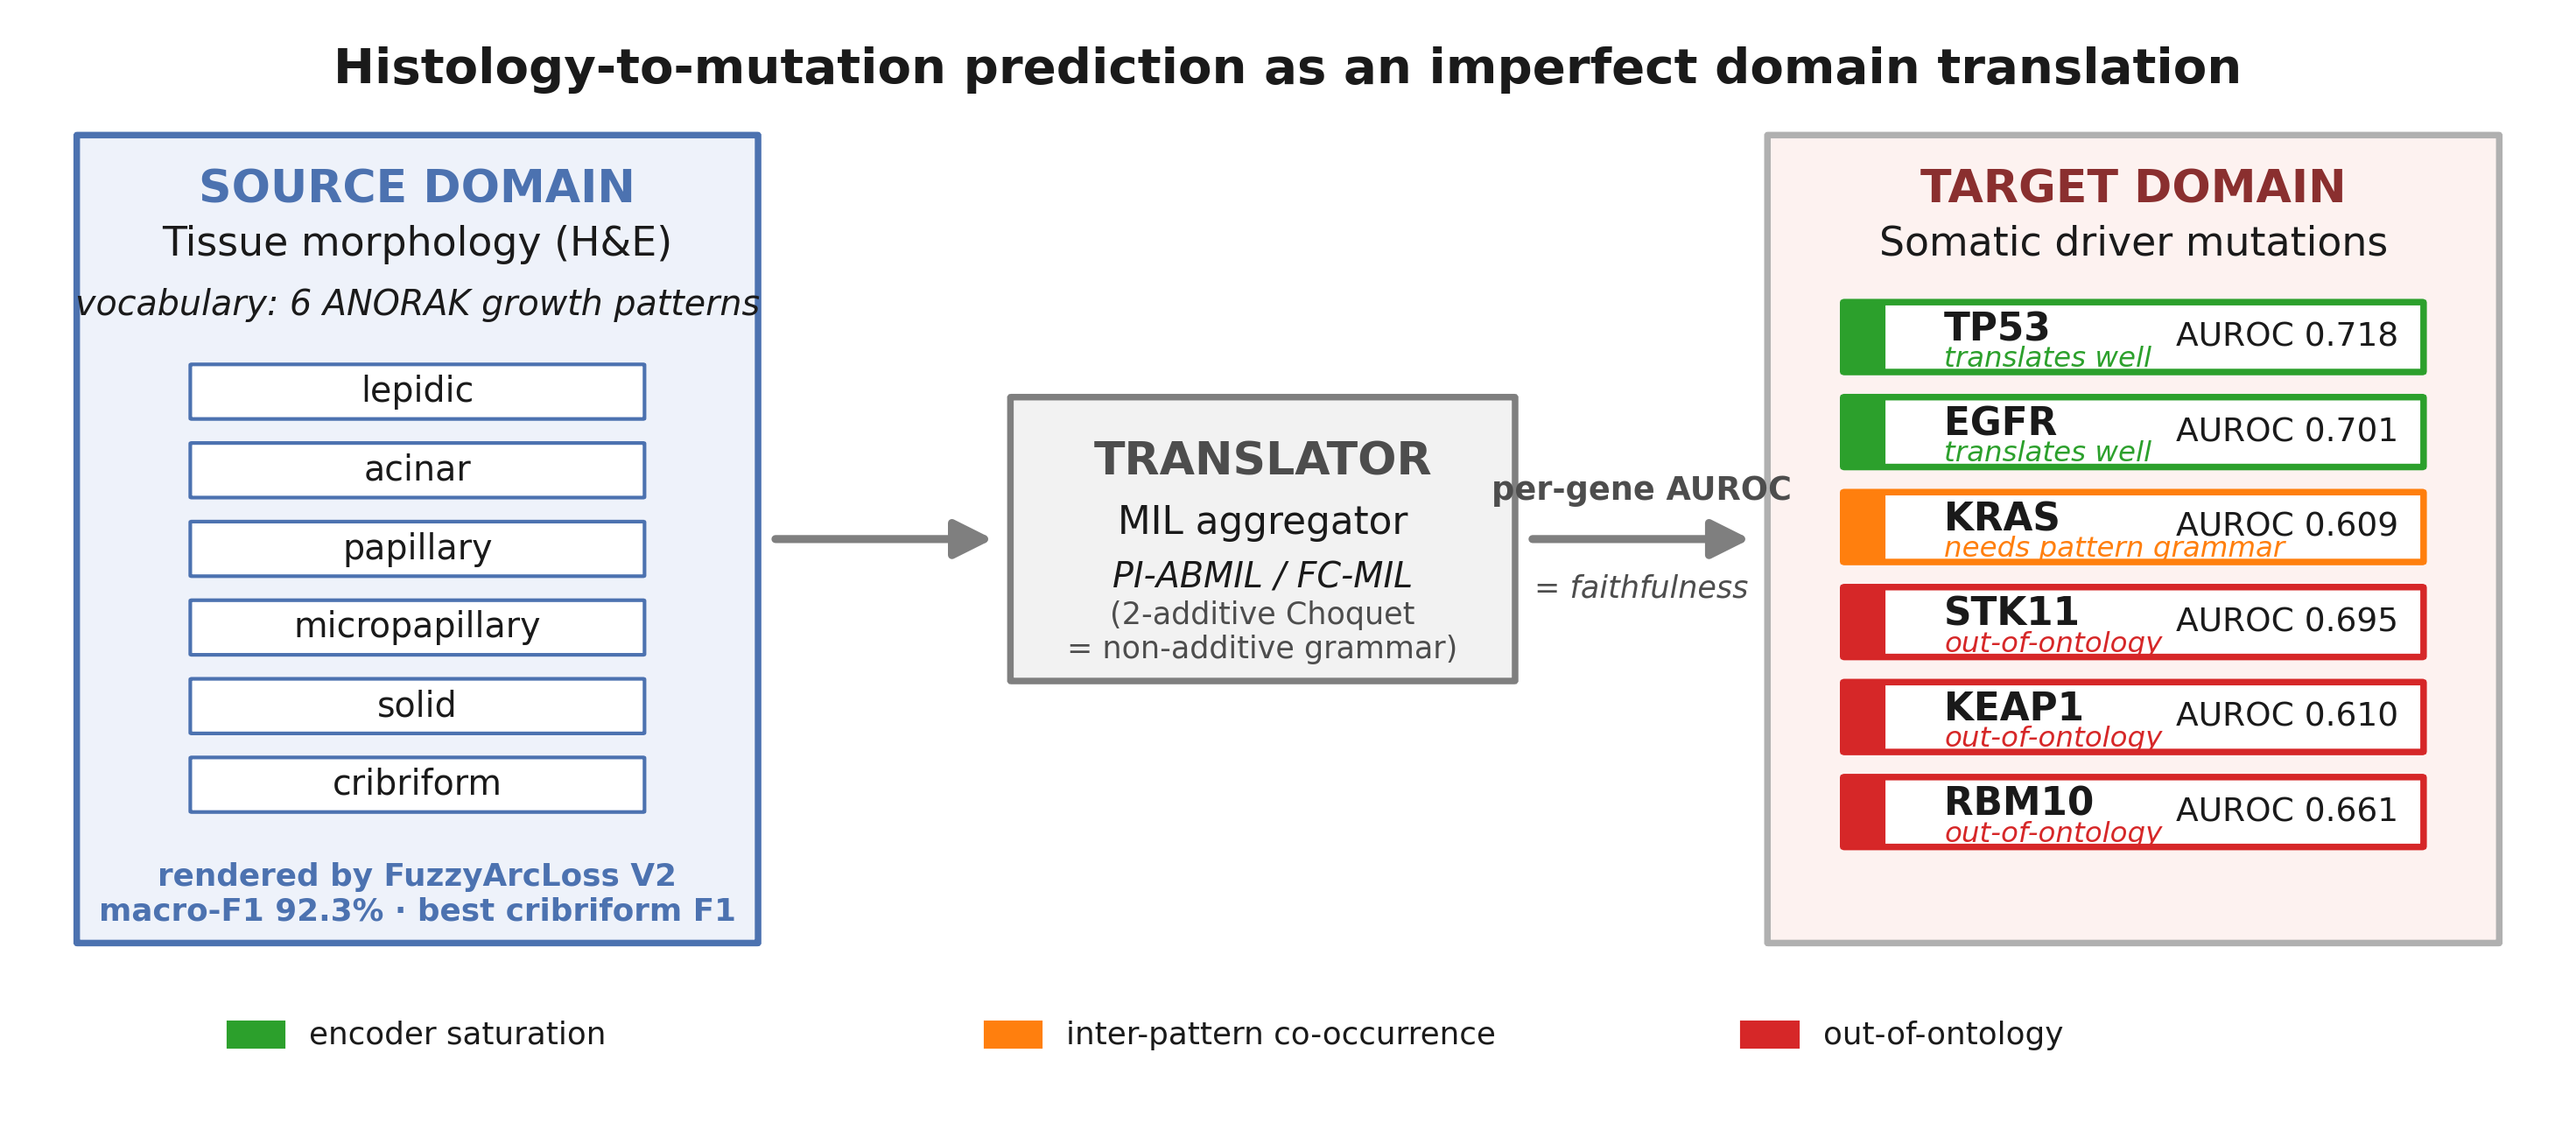
\includegraphics[width=\linewidth]{domain_translation_concept}
  \caption{\textbf{Cross-domain medical prediction as an imperfect
  translation, and the two channels over which it is decomposed.}
  \textbf{a}, A \emph{source} domain of tissue morphology, whose
  vocabulary is the six ANORAK growth patterns, is mapped by a
  multiple-instance translator onto a \emph{target} domain of somatic
  driver mutations; the per-target \auroc{} measures translational
  faithfulness averaged over the cohort. \textbf{b}, The two channels the
  aggregator receives. The morphology channel carries \ctranspath{} tile
  embeddings $\mathbf{h}_i$ into a gated-attention aggregator
  (\piabmil{}); the composition channel carries the $6$-d fuzzy pattern
  probabilities $\mathbf{p}_i$ into a $2$-additive Choquet integral
  (\fcmil{}). The two are disjoint until the classifier head, which is
  what makes \cref{eq:pid} well posed as a statement about two sources:
  neither channel can route information through the other, so an empty
  pattern-side atom cannot be an artefact of the architecture. Only the
  vocabulary and the encoder change when the framework moves to glioma MRI
  or to the electrocardiogram (\cref{fig:pipeline_glioma,fig:pipeline_ecg}).}
  \label{fig:framework}
\end{figure}

\FloatBarrier
% Scientific Reports Article Results (precedes the Discussion and the
% Methods in this build). Derived from 03_results_CM.tex and then pruned so
% that every main-text item is adequately powered and every claim is
% adjudicated:
%  - every deciding contrast of the regime rule is a main display item
%    (Table 2, tab:luad_contrasts);
%  - the KRAS conditional synergy test is one paragraph; its textbook
%    morphology figure is Supplementary Fig. fig:kras_lepidic_solid_proxy;
%  - the signal-tree taxonomy figure and the PID-regime mapping table are
%    Supplementary items (fig:signal_tree, tab:pid_regimes): the LUAD reads
%    are directional, so neither belongs among the headline results;
%  - the n~63 glioma pilot (IDH, 1p/19q, sex control) is Supplementary
%    Table tab:glioma_domainb and Supplementary Note 1; only the full-power
%    MGMT test stays in the main cross-domain table;
%  - the patient-sex control in LUAD is a row of Supplementary Table
%    tab:controls and is not discussed;
%  - the per-slide explanation tooling is described in Methods as released
%    software and is not a result.
%  Display items here: Table 1, Table 2, Table 3 (Fig. 1 is in the
%  Introduction).

\section*{Results}

\subsection*{One contrast resolves; the per-gene reads do not}

Quality filtering left $687$ analysable TCGA-LUAD images, but that
inventory is not a LUAD cohort: restricting to adenocarcinoma cases with
a mutation call and excluding solid-tissue-normal sections leaves $458$
tumour slides from $444$ patients across $33$ sites (Methods).
Prevalences span sevenfold, \textit{TP53} at $49.6\%$
to \textit{RBM10} at $7.0\%$.

Four conditions were ablated against a common \ctranspath{}
encoder\cite{wang2022ctranspath}: B2, \abmil{} on embeddings; B3,
\abmil{} on pattern probabilities; \piabmil{}, concat fusion; and
\fcmil{}, the $2$-additive Choquet head. Each ran under nested
cross-validation---early stopping on an inner split, the outer fold
scored once---across five seeds and two outer protocols, patient- and
site-preserved, for $1{,}200$ gene--condition--fold units. Contrasts are
adjudicated by a hierarchical bootstrap over seeds and patients,
site-clustered under the site protocol (Methods).

The resulting \auroc{} is low throughout
(\cref{tab:mutation_luad_resultssec}). \textit{TP53} is the only gene
whose embedding baseline clears $0.60$ under both protocols, and two
of six sit at or below $0.52$. \Cref{tab:luad_contrasts} reports every
contrast the regime rule reads---$48$ in all, four per gene under each
protocol---with its interval and the number of seeds on which its sign
holds. Exactly one contrast resolves: the
pattern channel alone is worse than the embedding alone---B3$-$B2
negative, interval excluding zero, same sign in all five seeds---on
\textit{TP53} and \textit{EGFR} under both protocols, \textit{STK11}
under one. None of the $36$ fusion contrasts
(\piabmil{}$-$B2, \fcmil{}$-$B2, \fcmil{}$-$\piabmil{}) excludes zero on
any gene under either protocol, and none falls inside the $\pm0.02$
equivalence margin either, so no gene can be read as saturated any more
than as complementary; \piabmil{} and \fcmil{} sit within a fold's
spread of B2 throughout and their per-seed signs disagree in $34$ of
the $36$ cells. A cohort-mean ranking of these architectures would be reading
noise.

\begin{table}[htbp]
\centering
% =====================================================================
% Table tab:mutation_luad — cohort v4, five seeds, two protocols.
%
% Source: results_luad_robustness_v4, 1200/1200 units aggregated
%   (5 seeds x 2 protocols x 6 genes x 4 conditions x 5 folds).
%   Point values: bootstrap_v4_final/luad_pooled_oof_aurocs_by_seed.csv,
%     pooled out-of-fold AUROC per seed, reported as mean +- SD across
%     the five seeds.
%   B3-B2 intervals: bootstrap_v4_final/luad_hierarchical_contrasts.csv,
%     hierarchical patient bootstrap (site-clustered under protocol b).
%
% NOTE(conditions): the v4 run scored B2, B3, PI and FC only. The former
%   B1 (XGBoost on the 7-d pattern vector) and A (one-hot ablation)
%   columns are not reproducible from this run and have been dropped
%   rather than carried over from the superseded cohort. See
%   TODO(b1-and-a) in 03_results_NMI.tex.
%
% Eight columns of mean$\pm$SD overflow the 166 mm text block at \small,
% so the table is wrapped in \resizebox exactly as
% tab_literature_comparison.tex is.
% =====================================================================
\resizebox{\linewidth}{!}{%
\small
\setlength{\tabcolsep}{4pt}
\renewcommand{\arraystretch}{1.15}
\begin{tabular}{l c c c c c c c}
\toprule
\textbf{Cond.} & \textbf{TP53} & \textbf{EGFR} & \textbf{STK11} &
\textbf{KEAP1} & \textbf{KRAS} & \textbf{RBM10} & \textbf{Mean} \\
 & {\scriptsize $n_+\!=\!220$} & {\scriptsize $67$} & {\scriptsize $58$}
 & {\scriptsize $79$} & {\scriptsize $124$} & {\scriptsize $30$} & \\
\midrule
\multicolumn{8}{l}{\textbf{a}, Patient-preserved outer folds}\\
\addlinespace[1pt]
B2 (ABMIL embeddings)
  & \textbf{.661}$\pm$.033 & \textbf{.582}$\pm$.060 & .591$\pm$.019
  & \textbf{.488}$\pm$.029 & \textbf{.517}$\pm$.026
  & .536$\pm$.047 & .562 \\
B3 (ABMIL patterns)
  & .579$\pm$.029 & .480$\pm$.023 & .499$\pm$.017
  & .485$\pm$.038 & .486$\pm$.031 & .490$\pm$.037 & .503 \\
PI-ABMIL (ours)
  & .658$\pm$.020 & .580$\pm$.046 & .578$\pm$.050
  & .446$\pm$.032 & .516$\pm$.025
  & \textbf{.552}$\pm$.027 & .555 \\
FC-MIL (ours)
  & .646$\pm$.031 & .567$\pm$.060 & \textbf{.608}$\pm$.021
  & .460$\pm$.020 & .506$\pm$.019 & .528$\pm$.038 & .553 \\
\addlinespace[2pt]
B3$-$B2 [95\% CI]
  & \textbf{$-$.082} & \textbf{$-$.102} & \textbf{$-$.092}
  & $-$.003 & $-$.031 & $-$.046 & \\
  & {\scriptsize[$-$.134,$-$.027]} & {\scriptsize[$-$.178,$-$.030]}
  & {\scriptsize[$-$.170,$-$.021]} & {\scriptsize[$-$.076,\,.070]}
  & {\scriptsize[$-$.094,\,.024]} & {\scriptsize[$-$.161,\,.073]} & \\
\midrule
\multicolumn{8}{l}{\textbf{b}, Site-preserved outer folds}\\
\addlinespace[1pt]
B2 (ABMIL embeddings)
  & \textbf{.640}$\pm$.024 & \textbf{.584}$\pm$.038
  & \textbf{.605}$\pm$.019 & .482$\pm$.021 & \textbf{.507}$\pm$.028
  & \textbf{.525}$\pm$.055 & .557 \\
B3 (ABMIL patterns)
  & .561$\pm$.032 & .485$\pm$.052 & .523$\pm$.044
  & \textbf{.488}$\pm$.059 & .475$\pm$.039 & .517$\pm$.045 & .508 \\
PI-ABMIL (ours)
  & .630$\pm$.043 & .576$\pm$.050 & .593$\pm$.024
  & .472$\pm$.019 & .502$\pm$.045 & .512$\pm$.057 & .547 \\
FC-MIL (ours)
  & .636$\pm$.026 & .557$\pm$.040 & .597$\pm$.056
  & .471$\pm$.015 & .501$\pm$.023 & .511$\pm$.071 & .546 \\
\addlinespace[2pt]
B3$-$B2 [95\% CI]
  & \textbf{$-$.079} & \textbf{$-$.099} & $-$.083
  & $+$.006 & $-$.032 & $-$.007 & \\
  & {\scriptsize[$-$.131,$-$.024]} & {\scriptsize[$-$.174,$-$.019]}
  & {\scriptsize[$-$.181,\,.001]} & {\scriptsize[$-$.067,\,.093]}
  & {\scriptsize[$-$.093,\,.035]} & {\scriptsize[$-$.103,\,.108]} & \\
\bottomrule
\end{tabular}%
}

\caption{\textbf{Mutation prediction on $458$ TCGA-LUAD slides from
$444$ patients, five seeds, two outer protocols.} Pooled out-of-fold
\auroc{}, mean $\pm$ SD across seeds, under nested cross-validation.
B2~$=$~\abmil{} on \ctranspath{} embeddings (the ceiling baseline);
B3~$=$~\abmil{} on pattern probabilities only; PI~$=$~\piabmil{} concat
fusion; FC~$=$~\fcmil{} $2$-additive Choquet. Best per gene in bold.
The B3$-$B2 rows give the hierarchical bootstrap interval over seeds and
patients, site-clustered in \textbf{b}; bold marks the genes on
which it excludes zero---\textit{TP53}, \textit{EGFR} and \textit{STK11}
in \textbf{a}, and only \textit{TP53} and \textit{EGFR} in \textbf{b},
where the \textit{STK11} interval reaches $+0.001$---and these are the
only resolved contrasts in the
table. No fusion contrast (\piabmil{}$-$B2, \fcmil{}$-$B2,
\fcmil{}$-$\piabmil{}) resolves on any gene under either protocol, and
no equivalence is established either, at the $\pm0.02$ margin the
regime reads require (\cref{tab:luad_contrasts,tab:design_power}).}
\label{tab:mutation_luad_resultssec}
\end{table}

\begin{table}[htbp]
\centering
% Generated by scripts/make_contrasts_table.py from
% data/luad_hierarchical_contrasts.csv. Do not edit by hand.
\resizebox{\linewidth}{!}{%
\small
\setlength{\tabcolsep}{4pt}
\renewcommand{\arraystretch}{1.2}
\begin{tabular}{l l l l l}
\toprule
\textbf{Gene} & \textbf{$\mathrm{PI}-\mathrm{B2}$} & \textbf{$\mathrm{FC}-\mathrm{B2}$} & \textbf{$\mathrm{FC}-\mathrm{PI}$} & \textbf{$\mathrm{B3}-\mathrm{B2}$} \\
 & {\scriptsize (ii-a) additive} & {\scriptsize equivalence, (i)/(iii)} & {\scriptsize (ii-b) non-additive} & {\scriptsize what the vocabulary omits} \\
\midrule
\multicolumn{5}{l}{\textbf{a}, Patient-preserved outer folds}\\
\addlinespace[1pt]
\textit{TP53} & $-$.003 {\scriptsize[$-$.029,\,$+$.022]} {\scriptsize 2/5} & $-$.015 {\scriptsize[$-$.042,\,$+$.010]} {\scriptsize 2/5} & $-$.012 {\scriptsize[$-$.045,\,$+$.020]} {\scriptsize 2/5} & \textbf{$-$.082} {\scriptsize[$-$.134,\,$-$.026]} {\scriptsize 0/5} \\
\textit{EGFR} & $-$.002 {\scriptsize[$-$.045,\,$+$.041]} {\scriptsize 3/5} & $-$.015 {\scriptsize[$-$.073,\,$+$.040]} {\scriptsize 2/5} & $-$.013 {\scriptsize[$-$.071,\,$+$.040]} {\scriptsize 2/5} & \textbf{$-$.102} {\scriptsize[$-$.178,\,$-$.030]} {\scriptsize 0/5} \\
\textit{STK11} & $-$.013 {\scriptsize[$-$.065,\,$+$.034]} {\scriptsize 3/5} & $+$.018 {\scriptsize[$-$.027,\,$+$.064]} {\scriptsize 4/5} & $+$.030 {\scriptsize[$-$.026,\,$+$.090]} {\scriptsize 3/5} & \textbf{$-$.092} {\scriptsize[$-$.170,\,$-$.021]} {\scriptsize 0/5} \\
\textit{KEAP1} & $-$.042 {\scriptsize[$-$.096,\,$+$.008]} {\scriptsize 1/5} & $-$.028 {\scriptsize[$-$.082,\,$+$.034]} {\scriptsize 1/5} & $+$.014 {\scriptsize[$-$.038,\,$+$.077]} {\scriptsize 3/5} & $-$.003 {\scriptsize[$-$.076,\,$+$.070]} {\scriptsize 3/5} \\
\textit{KRAS} & $-$.001 {\scriptsize[$-$.042,\,$+$.037]} {\scriptsize 2/5} & $-$.011 {\scriptsize[$-$.057,\,$+$.036]} {\scriptsize 1/5} & $-$.010 {\scriptsize[$-$.045,\,$+$.022]} {\scriptsize 0/5} & $-$.031 {\scriptsize[$-$.094,\,$+$.024]} {\scriptsize 2/5} \\
\textit{RBM10} & $+$.016 {\scriptsize[$-$.046,\,$+$.081]} {\scriptsize 4/5} & $-$.008 {\scriptsize[$-$.091,\,$+$.076]} {\scriptsize 2/5} & $-$.024 {\scriptsize[$-$.099,\,$+$.044]} {\scriptsize 1/5} & $-$.046 {\scriptsize[$-$.160,\,$+$.073]} {\scriptsize 1/5} \\
\midrule
\multicolumn{5}{l}{\textbf{b}, Site-preserved outer folds, site-clustered bootstrap}\\
\addlinespace[1pt]
\textit{TP53} & $-$.010 {\scriptsize[$-$.051,\,$+$.022]} {\scriptsize 3/5} & $-$.004 {\scriptsize[$-$.033,\,$+$.026]} {\scriptsize 1/5} & $+$.006 {\scriptsize[$-$.028,\,$+$.042]} {\scriptsize 3/5} & \textbf{$-$.079} {\scriptsize[$-$.131,\,$-$.024]} {\scriptsize 0/5} \\
\textit{EGFR} & $-$.008 {\scriptsize[$-$.045,\,$+$.026]} {\scriptsize 2/5} & $-$.027 {\scriptsize[$-$.098,\,$+$.043]} {\scriptsize 1/5} & $-$.019 {\scriptsize[$-$.080,\,$+$.050]} {\scriptsize 1/5} & \textbf{$-$.099} {\scriptsize[$-$.174,\,$-$.019]} {\scriptsize 0/5} \\
\textit{STK11} & $-$.012 {\scriptsize[$-$.060,\,$+$.029]} {\scriptsize 2/5} & $-$.008 {\scriptsize[$-$.069,\,$+$.053]} {\scriptsize 2/5} & $+$.005 {\scriptsize[$-$.056,\,$+$.062]} {\scriptsize 3/5} & $-$.083 {\scriptsize[$-$.181,\,$+$.001]} {\scriptsize 0/5} \\
\textit{KEAP1} & $-$.010 {\scriptsize[$-$.040,\,$+$.015]} {\scriptsize 0/5} & $-$.012 {\scriptsize[$-$.053,\,$+$.033]} {\scriptsize 2/5} & $-$.001 {\scriptsize[$-$.043,\,$+$.043]} {\scriptsize 3/5} & $+$.006 {\scriptsize[$-$.067,\,$+$.093]} {\scriptsize 3/5} \\
\textit{KRAS} & $-$.004 {\scriptsize[$-$.045,\,$+$.038]} {\scriptsize 2/5} & $-$.005 {\scriptsize[$-$.050,\,$+$.041]} {\scriptsize 2/5} & $-$.001 {\scriptsize[$-$.048,\,$+$.042]} {\scriptsize 2/5} & $-$.032 {\scriptsize[$-$.092,\,$+$.035]} {\scriptsize 1/5} \\
\textit{RBM10} & $-$.013 {\scriptsize[$-$.109,\,$+$.127]} {\scriptsize 1/5} & $-$.014 {\scriptsize[$-$.113,\,$+$.127]} {\scriptsize 2/5} & $-$.001 {\scriptsize[$-$.063,\,$+$.082]} {\scriptsize 2/5} & $-$.007 {\scriptsize[$-$.103,\,$+$.108]} {\scriptsize 3/5} \\
\bottomrule
\end{tabular}%
}

\caption{\textbf{Every contrast the regime rule reads, with its
interval.} For each gene and outer protocol, the four between-condition
contrasts of the noise-aware rule (Methods): \piabmil{}$-$B2 decides
additive complementarity (ii-a); \fcmil{}$-$B2 together with
\piabmil{}$-$B2 must fall inside $\pm0.02$ for an equivalence read of
regime (i) or (iii); \fcmil{}$-$\piabmil{} decides the non-additive
sub-form (ii-b); and B3$-$B2 measures what the vocabulary omits. Each
cell gives the pooled out-of-fold point contrast, its $95\%$
hierarchical-bootstrap interval over seeds and patients ($2{,}000$
draws; site-clustered in \textbf{b}), and the number of the five seeds
on which the point contrast is positive. Bold marks an interval
excluding zero; a superscript $\approx$ would mark an interval inside
the $\pm0.02$ equivalence margin, and no cell earns one. Of $48$
contrasts, five exclude zero and all five are B3$-$B2; none of the $36$
fusion contrasts does, and none is equivalent to zero, which is why
every LUAD regime read is reported as directional and unadjudicated.
Generated from the same bootstrap output as the B3$-$B2 rows of
\cref{tab:mutation_luad_resultssec}.}
\label{tab:luad_contrasts}
\end{table}

\subsection*{The pipeline is calibrated and its ceiling is low}

Controls ran on three seeds under both protocols
(\cref{tab:controls}). Permuting
\textit{TP53} labels across patients returns $0.496\pm0.010$ on B2 and
$0.487\pm0.015$ on B3, so nothing in the protocol manufactures
discrimination. That the pipeline learns is established independently of
every mutation label: separating the $458$ tumour slides from the $62$
solid-tissue-normal sections the cohort excludes reaches
$0.976\pm0.004$ on B2 and $0.968\pm0.013$ site-preserved. The pattern
channel clears chance too ($0.800\pm0.022$), so the ANORAK head is
functional: its near-chance mutation values are an absent signal, not
a broken classifier. \textit{TP53} then replicates the main arm on fresh
seeds ($0.672\pm0.032$) without having to certify the pipeline that
produced it. A cohort separable at $0.98$ on morphology stops at $0.66$
on genotype.

\subsection*{Three kinds of failure behind one Inconclusive label}

Read alongside the per-gene biology, the six genes point towards two of
the three regimes rather than onto a scale; the directions are given
here, the adjudication in \cref{tab:luad_contrasts} confirms none of
them, and no gene points towards regime~(ii).
The full taxonomy, with each gene's directional read and its
adjudication status, is drawn in \cref{fig:signal_tree}, and the
mapping of each regime onto an atom of \cref{eq:pid} is in
\cref{tab:pid_regimes}.

\paragraph{Encoder saturation, regime~(i): TP53 and EGFR.}
The embedding-only baseline B2 reaches $0.661$ and $0.582$ under
patient-preserved folds; fusion moves the \auroc{} by $\leq0.02$ in
point estimate, while the pattern channel alone falls $0.082$ and
$0.102$ below the embedding. That is the predicted signature when the
encoder already carries what the vocabulary names---TP53's high-grade
nuclear pleomorphism, EGFR's lepidic-leaning low-grade phenotype. But
the read requires an \emph{equivalence}: that fusion adds nothing, not
merely that it appears to. Neither \piabmil{}$-$B2 nor \fcmil{}$-$B2
falls inside the $\pm0.02$ band under either protocol, so the saturation
read is directional and unadjudicated, and \textit{EGFR}, at
$0.582\pm0.060$, carries the widest spread of any embedding baseline.

\paragraph{Complementarity, regime~(ii): tested on KRAS and not
supported.} The Choquet head learns a positive
$I(\text{lepidic}\!\times\!\text{solid})\!=\!{+}0.032$ against a negative
$I(\text{lepidic}\!\times\!\text{micropapillary})\!=\!-0.018$, and the
pair it selects is the histological proxy for invasive mucinous
adenocarcinoma, the KRAS-enriched
subtype\cite{rekhtman2013krassolid} (\cref{fig:kras_lepidic_solid_proxy}).
The regime claim is stronger than that agreement: that the Choquet head
buys accuracy \emph{because} the two patterns co-occur. A cohort-wide
contrast cannot test a conditional statement, so we cut the $444$
patients into terciles of per-slide co-activation
$\min(f_{\text{lep}}, f_{\text{sol}})$, using no mutation-side quantity.
The premise holds only weakly: the pair co-occurs in $452$ of $458$
slides but at low magnitude (median $0.005$), so there is no discrete
subpopulation to isolate, although co-activation does track KRAS
descriptively ($\auroc\!=\!0.582$; prevalence rising from $22.3\%$ to
$33.1\%$ across terciles, risk ratio $1.56$ $[1.07,\,2.29]$). The
conditional test returns nothing (\cref{tab:kras_coactivation}): no
stratum interval excludes zero under either protocol, and the
high${-}$low difference is $-0.024$ $[-0.117,\,{+}0.072]$
patient-preserved and ${+}0.025$ $[-0.090,\,{+}0.141]$
site-preserved---unresolved in both and disagreeing in sign, the
pattern of no effect rather than of an effect too small to see. Two
bounds explain that: at $n\!=\!444$ the design resolves only $0.135$
\auroc{} ($0.165$ site-preserved) at $80\%$ power, several times any
aggregator gain reported in this literature ($0.008$--$0.046$,
\cref{tab:literature_power_audit}), and there was no gain to localise,
since \fcmil{} scores $0.506$ on KRAS. The synergy cell is left empty.
What survives is the morphological association, which the model does
not convert: the hand-computed co-activation feature tracks KRAS better
than the trained aggregator. That ordering admits two readings---a
synergy the Choquet head fails to convert, or a marginal association no
head would---and the cohort cannot separate them: the first is a claim
about the aggregator's hypothesis space, and the stratified contrast
that would test it is the one \cref{tab:design_power} puts beyond
roughly $9{,}000$ patients. The alternative is reported as untested,
not excluded.

\paragraph{Out-of-ontology, regime~(iii): STK11, with KEAP1 and RBM10
below it.} For these three the pattern channel converts into no usable
gain, for three different reasons, and only the first is
out-of-ontology in the intended sense. STK11 (best $0.608$) is a
\emph{label-space mismatch}: the embedding carries signal the vocabulary
does not, B3 falling $0.092$ below B2 with an interval excluding zero,
its driver being an immune-cold
microenvironment\cite{skoulidis2018stk11pd1} that an ontology built for
tumour-cell growth patterns cannot name. KEAP1 is a stronger null than
the regime allows: every condition sits at or below $0.49$ under both
protocols, so the NRF2 oxidative-stress
axis\cite{li2011keap1papillary} is invisible not merely to the
vocabulary but to the encoder---the LUAD analogue of the MGMT result
below. RBM10 (best $0.552$) is a \emph{collapse to prior} at
$n_+\!=\!30$, where the across-seed spread exceeds every contrast we
would want to read.

This is where the decomposition earns its place: in separating kinds of
failure that a leaderboard reports as one number. KEAP1 and RBM10 sit
within $0.05$ \auroc{} on B2 and both would be called
Inconclusive, yet they prescribe opposite next experiments. KEAP1's
pattern side is empty and so is its embedding side---both channels at or
below $0.49$ under both protocols---so more LUAD slides will not help
and the deficit is the source modality. RBM10 is unestimable rather than
empty: at $n_+\!=\!30$ its across-seed spread of $\pm0.027$ to
$\pm0.071$ swamps the $\pm0.02$ contrasts, so the deficit is cohort
size. KRAS adds a third kind, its pattern side
tracking the target while the aggregator that should exploit it sits at
chance. One Inconclusive label thus covers three states---empty,
unestimable, unconverted---calling for a new modality, a larger cohort,
and one larger by an order of magnitude (\cref{tab:design_power}).

\subsection*{The procedure transfers; the predictor does not}

Nothing in the decomposition is specific to histology, so we ran the
identical four conditions, directional rule and threshold in two further
modalities and across cohorts within one
(\cref{tab:crossdomain_merged}); only the vocabulary and the encoder
change.

In \textbf{glioma MRI}, the VASARI controlled
terminology\cite{gutman2013vasari} replaces ANORAK, and the target is
the one a decade of work has failed to predict. MGMT is an
\emph{encoder-ceiling} test, and the distinction is
load-bearing. The balanced BraTS cohort ($n\!=\!577$, ${\sim}52\%$
methylated) excludes a data floor outright, and every condition sits at
chance ($0.52$--$0.55$ over five seeds; the upper bound of the best,
$0.59$, is below the $0.70$ threshold), so the verdict is Inconclusive and is resolved at
full power: the instrument declines to certify the best-documented
untranslatable target in medical machine learning. The regime is read
from those levels, not from a contrast. The fusion contrasts have
half-widths near $0.04$ under the seed-and-patient bootstrap and resolve
nothing at the $\pm0.02$ margin
(\cref{tab:crossdomain_contrasts}), so what $577$ cases establish is that
no reader of this modality in the design reaches the target---the
modality-ceiling form of (iii)---and not that fusion equals the
encoder, which would need roughly $2{,}500$ cases to certify. The VASARI
channel here is propagated rather than expert-scored, so the two sources
are not independent readings and the strict empty-atom separation real
VASARI licenses does not apply. The null establishes that the target is
unreachable from this modality by this encoder---not a falsification of
the two-source framework, which this arm cannot test (Methods). A pilot on
the $n\!\sim\!63$ TCGA-LGG subjects with expert-scored VASARI (IDH,
1p/19q, a sex control) is reported in \cref{tab:glioma_domainb} and
Supplementary Note~1; at that size its reads are directional only and
we draw no regime from them.

In the \textbf{electrocardiogram}, the $71$ graded SCP-ECG statements of
PTB-XL\cite{wagner2020ptbxl} supply an already-fuzzy vocabulary.
Patient sex and age are recorded for every case and are not derivable
from the statements, so they furnish a leakage-free pair. Both are
Conclusive, and both meet the equivalence condition of the noise-aware
rule: $\mathrm{PI}-\mathrm{B2}$ and $\mathrm{FC}-\mathrm{B2}$ fall inside
$\pm0.02$ with intervals of half-width ${\approx}0.008$ over five seeds
and $18{,}869$
patients, so regime~(i) is adjudicated here---the one cohort in this
work large enough to certify it---with the encoder-saturated signature
that TP53 and EGFR show directionally in LUAD. Both fusion contrasts
are $+0.003$ on both targets with upper bounds of $+0.011$
(\cref{tab:crossdomain_contrasts}): no gain
excludes zero and none approaches the $0.02$ this literature claims for
an aggregator change, so it is equivalence, not complementarity. No
statement pair across all $\binom{71}{2}$ moves \fcmil{} off additive
fusion ($\fcmil{}-\piabmil{}$ $-0.003$ and $-0.000$): the negative
result the model-side signature is designed to report.

Across \textbf{cohorts}, the frozen TCGA-trained pipeline applied
off-the-shelf to CPTAC-LUAD gives a clean negative. \textit{TP53}'s
\auroc{} falls from $0.661$ to
$0.53$ ($95\%$ CI $0.42$--$0.64$), an interval excluding the TCGA point
estimate; Reinhard stain normalisation does not recover it, so a global
colour cast is not the driver. Both cohorts return Inconclusive, so what
the transfer establishes is not a change of verdict but that the value
itself does not survive the move. Re-fitting the
four conditions inside CPTAC with only the representation carried over
reaches \textit{TP53} $0.698$, marginally \emph{above} the TCGA value,
with the encoder-only baselines agreeing to $0.004$---so the coupling is
present in the second cohort at full strength and what failed is the
transported decision function alone. The
regime stays unresolved: the deciding contrast spans zero, and
separating two fitted conditions is a stricter demand than fitting
either, which $106$ patients do not meet (\cref{tab:cptac_refit}).

\begin{table}[htbp]
\centering
% Table tab:crossdomain_merged — main Table 3 (Scientific Reports build).
% Levels only: pooled OOF AUROC per condition with its 95% hierarchical
% (five seeds x patients) bootstrap interval, verdict and regime. The
% contrasts the regime rule reads are Table 4 (tab_crossdomain_contrasts_SR).
% The n~63 glioma pilot rows (IDH, 1p/19q, sex control) are Supplementary
% Table tab:glioma_domainb and Supplementary Note 1; per-gene CPTAC transfer
% values and the stain/field-of-view controls are Supplementary Tables.
\footnotesize
\setlength{\tabcolsep}{5pt}
\renewcommand{\arraystretch}{1.15}
\begin{tabular}{l cccc l l}
\toprule
\textbf{Target} & \textbf{B2} & \textbf{B3} & \textbf{PI} & \textbf{FC} &
  \textbf{Verdict} & \textbf{Regime} \\
 & encoder & vocabulary & concat & Choquet & & \\
\midrule
\multicolumn{7}{l}{\emph{(a) Glioma MRI $\rightarrow$ MGMT methylation.}
  VASARI semantic MR features; BraTS~2021, $n\!=\!577$} \\
\addlinespace[2pt]
MGMT\textsuperscript{$\dagger$} &
  \makecell{$0.539$\\{[}0.50, 0.58{]}} &
  \makecell{$0.519$\\{[}0.48, 0.56{]}} &
  \makecell{$0.525$\\{[}0.48, 0.57{]}} &
  \makecell{$\mathbf{0.552}$\\{[}0.51, 0.59{]}} &
  Inconclusive & (iii) modality ceiling \\
\addlinespace[2pt]
\midrule
\multicolumn{7}{l}{\emph{(b) Electrocardiogram $\rightarrow$ physiological
  state.} $71$ graded SCP-ECG statements; PTB-XL, $21{,}799$ records,
  $18{,}869$ patients} \\
\addlinespace[2pt]
Sex &
  \makecell{$0.884$\\{[}0.877, 0.892{]}} &
  \makecell{$0.612$\\{[}0.604, 0.621{]}} &
  \makecell{$\mathbf{0.888}$\\{[}0.883, 0.893{]}} &
  \makecell{$0.885$\\{[}0.880, 0.891{]}} &
  Conclusive & (i) encoder-saturated \\
\addlinespace[3pt]
Age $\geq 65$ &
  \makecell{$0.825$\\{[}0.817, 0.834{]}} &
  \makecell{$0.732$\\{[}0.725, 0.739{]}} &
  \makecell{$\mathbf{0.828}$\\{[}0.822, 0.833{]}} &
  \makecell{$\mathbf{0.828}$\\{[}0.821, 0.835{]}} &
  Conclusive & (i) encoder-saturated \\
\addlinespace[2pt]
\midrule
\multicolumn{7}{l}{\emph{(c) Cohort transfer, TCGA-LUAD $\rightarrow$
  CPTAC-LUAD.} \textit{TP53}, the one gene clearing the estimation
  floor ($n_+\!=\!55$)} \\
\addlinespace[2pt]
Frozen pipeline & \multicolumn{4}{c}{$0.53$ \ [0.42, 0.64]; \ $0.48$ after
  stain normalisation} & Inconclusive & not testable\textsuperscript{$\ddagger$} \\
\addlinespace[2pt]
Re-fitted in CPTAC & $0.665$ & $0.667$ & $\mathbf{0.698}$ & $0.669$ &
  Inconclusive & unresolved\textsuperscript{$\S$} \\
\bottomrule
\end{tabular}
\begin{flushleft}\footnotesize
Panels \textbf{a} and \textbf{b}: pooled out-of-fold $\auroc$ over five
patient-disjoint folds and five seeds, with its $95\%$ hierarchical
bootstrap interval ($2{,}000$ draws resampling seeds and then patients,
as in LUAD; in \textbf{b} all records of a resampled patient travel
together). Conditions as in LUAD: $\mathrm{B2}$ encoder only,
$\mathrm{B3}$ source vocabulary only, $\mathrm{PI}$ concat fusion,
$\mathrm{FC}$ encoder $+$ $2$-additive Choquet over the vocabulary; best
per target in bold. The \emph{Verdict} thresholds the level at $0.70$;
the \emph{Regime} is read from the between-condition contrasts of
\cref{tab:crossdomain_contrasts}, never from the largest cell.
\textsuperscript{$\dagger$}MGMT is scored on the balanced BraTS~2021
cohort (${\sim}52\%$ methylated). The verdict is resolved at full power:
the upper bound of the best condition ($0.59$) lies below $0.70$. The
regime is the one case read from levels rather than from a contrast:
every condition, the encoder alone included, sits at chance, which is the
modality-ceiling form of (iii) (Methods). The VASARI channel is
propagated from the annotated seed rather than expert-scored, so the
claim rests on the unconstrained encoder remaining at chance, not on the
strict empty-atom separation that expert VASARI licenses. The
$n\!\sim\!63$ TCGA-LGG pilot with expert-scored VASARI (IDH, 1p/19q, sex
control) is \cref{tab:glioma_domainb}.
\textbf{(c)}~$498$ slides from $106$ genotyped CPTAC patients; $95\%$
CI from $2{,}000$ patient resamples.
\textsuperscript{$\ddagger$}The frozen arm applies one transported
predictor per gene and therefore cannot express a regime, which is a
contrast across four conditions; it tests the decision function, not the
assignment.
\textsuperscript{$\S$}Re-fitting the four conditions inside CPTAC with
only the representation carried over reaches \textit{TP53} $0.698$
against the TCGA value of $0.661$, so the morphology-to-genotype coupling
is present in the second cohort and the off-the-shelf collapse is a
property of the transported decision function. The deciding contrast
$\piabmil{}-\mathrm{B2}$ is $+0.032$ with a $95\%$ CI of $-0.041$ to
$+0.102$, which spans zero, so no regime is asserted. Per-gene transfer
values and the stain-normalisation and field-of-view controls are in
\cref{tab:cptac_transfer,tab:cptac_refit}.
\end{flushleft}

\caption{\textbf{The procedure run unchanged in two further modalities
and across cohorts.} \textbf{a}, Glioma MRI\,$\rightarrow$\,MGMT
promoter methylation with the VASARI vocabulary: the verdict is resolved
at full power and the regime is read from levels.
\textbf{b}, Electrocardiogram\,$\rightarrow$\,physiological
state with the graded SCP-ECG statements: the one cohort in which the
equivalence condition of the rule is met. \textbf{c}, Cohort transfer from
TCGA-LUAD to CPTAC-LUAD. Only the vocabulary and the encoder change
between panels; the four conditions, the directional regime rule and the
Conclusive/Inconclusive threshold are identical throughout, which is the
precise sense in which the procedure rather than the model transfers.
The contrasts from which the regimes are read are
\cref{tab:crossdomain_contrasts}.}
\label{tab:crossdomain_merged}
\end{table}

\begin{table}[htbp]
\centering
% Table tab:crossdomain_contrasts — main Table 4 (Scientific Reports build).
% The four between-condition contrasts the noise-aware rule reads, for the
% three full-power cross-domain targets of Table 3, from
% data/glioma_mgmt_bootstrap_contrasts.csv and data/ecg_bootstrap_contrasts.csv
% (hierarchical bootstrap, five seeds x patients, 2,000 draws).
\footnotesize
\setlength{\tabcolsep}{6pt}
\renewcommand{\arraystretch}{1.15}
\begin{tabular}{l l r l c c c}
\toprule
\textbf{Contrast} & \textbf{What it decides} & \textbf{Estimate} &
  \textbf{95\% CI} & \textbf{Excludes 0} & \textbf{Within $\pm0.02$} &
  \textbf{Seeds $>0$} \\
\midrule
\multicolumn{7}{l}{\emph{(a) MGMT, BraTS~2021, $n\!=\!577$}} \\
\addlinespace[2pt]
$\mathrm{PI}-\mathrm{B2}$ & (ii-a) additive gain; equivalence gate &
  $-0.015$ & $[-0.057,\ +0.028]$ & no & no & 2/5 \\
$\mathrm{FC}-\mathrm{B2}$ & equivalence gate &
  $+0.012$ & $[-0.021,\ +0.048]$ & no & no & 4/5 \\
$\mathrm{FC}-\mathrm{PI}$ & (ii-b) non-additive gain &
  $+0.027$ & $[-0.013,\ +0.066]$ & no & no & 5/5 \\
$\mathrm{B3}-\mathrm{B2}$ & what the vocabulary omits &
  $-0.021$ & $[-0.072,\ +0.032]$ & no & no & 0/5 \\
\addlinespace[2pt]
\midrule
\multicolumn{7}{l}{\emph{(b) Sex, PTB-XL, $18{,}869$ patients}} \\
\addlinespace[2pt]
$\mathrm{PI}-\mathrm{B2}$ & (ii-a) additive gain; equivalence gate &
  $+0.003$ & $[-0.003,\ +0.011]$ & no & \textbf{yes} & 4/5 \\
$\mathrm{FC}-\mathrm{B2}$ & equivalence gate &
  $+0.000$ & $[-0.006,\ +0.007]$ & no & \textbf{yes} & 3/5 \\
$\mathrm{FC}-\mathrm{PI}$ & (ii-b) non-additive gain &
  $-0.003$ & $[-0.007,\ +0.002]$ & no & \textbf{yes} & 1/5 \\
$\mathrm{B3}-\mathrm{B2}$ & what the vocabulary omits &
  $\mathbf{-0.272}$ & $[-0.283,\ -0.262]$ & \textbf{yes} & no & 0/5 \\
\addlinespace[2pt]
\midrule
\multicolumn{7}{l}{\emph{(c) Age $\geq 65$, PTB-XL, $18{,}869$ patients}} \\
\addlinespace[2pt]
$\mathrm{PI}-\mathrm{B2}$ & (ii-a) additive gain; equivalence gate &
  $+0.003$ & $[-0.006,\ +0.011]$ & no & \textbf{yes} & 3/5 \\
$\mathrm{FC}-\mathrm{B2}$ & equivalence gate &
  $+0.003$ & $[-0.006,\ +0.011]$ & no & \textbf{yes} & 2/5 \\
$\mathrm{FC}-\mathrm{PI}$ & (ii-b) non-additive gain &
  $-0.000$ & $[-0.005,\ +0.005]$ & no & \textbf{yes} & 2/5 \\
$\mathrm{B3}-\mathrm{B2}$ & what the vocabulary omits &
  $\mathbf{-0.093}$ & $[-0.104,\ -0.084]$ & \textbf{yes} & no & 0/5 \\
\bottomrule
\end{tabular}
\begin{flushleft}\footnotesize
Each contrast is the difference of pooled out-of-fold $\auroc$ between two
conditions of \cref{tab:crossdomain_merged}, with a $95\%$ interval from
$2{,}000$ hierarchical draws (seeds with replacement, then patients within
each drawn seed). \emph{Excludes 0}: the interval does not contain zero.
\emph{Within $\pm0.02$}: the whole interval lies inside the equivalence
margin, the condition under which the rule declares a difference absent.
\emph{Seeds $>0$}: seeds, of five, in which the point estimate is
positive. Rows are in the order the rule reads them (Methods).
\textbf{(a)}~MGMT resolves nothing by contrast: half-widths near $0.04$
exceed the margin, so equivalence is not certified and
$\mathrm{FC}-\mathrm{PI}=+0.027$, positive in all five seeds yet spanning
zero, is not promoted; certifying equivalence would need roughly
$2{,}500$ cases. The regime in \cref{tab:crossdomain_merged} is therefore
read from levels (all four upper bounds below $0.70$), the one target in
this work to which that clause applies.
\textbf{(b, c)}~Both ECG targets meet the equivalence condition,
$\mathrm{PI}-\mathrm{B2}$ and $\mathrm{FC}-\mathrm{B2}$ inside $\pm0.02$,
so regime~(i) is adjudicated here rather than read from means: the only
cohort in this work large enough to do so. Once seed variance enters the
interval no fusion contrast excludes zero on either target (upper bounds
$+0.011$), so the margin is not even approached: equivalence, not
complementarity. The $2$-additive Choquet head emits an interaction index
over all $\binom{71}{2}$ statement pairs and none lets $\mathrm{FC}$
improve on $\mathrm{PI}$, so the synergy channel is empty, a measured
negative at this sample size rather than a deferral. The large negative
$\mathrm{B3}-\mathrm{B2}$ on both targets is what separates (i) from
(iii): the vocabulary omits most of what the encoder reads.
\end{flushleft}

\caption{\textbf{Every contrast the regime rule reads in the cross-domain
arms, with its interval.} The counterpart of \cref{tab:luad_contrasts}
for the three full-power targets of \cref{tab:crossdomain_merged}:
\textbf{a}, MGMT, where no contrast resolves and the regime is read from
levels; \textbf{b}, \textbf{c}, sex and age from the electrocardiogram,
where both fusion-versus-encoder contrasts fall inside the $\pm0.02$
equivalence margin and regime~(i) is adjudicated.}
\label{tab:crossdomain_contrasts}
\end{table}

\FloatBarrier
% Scientific Reports Article Discussion: continuous prose without
% subheadings, no display items; the final paragraph states what is
% established, what is a design argument and what is open. Derived from
% 04_discussion_CM.tex. Relocated rather than deleted:
%   - PID literature positioning and the differentiation from Liang et al.
%     -> Methods, "Relation to prior information-decomposition work"
%   - the noise-aware estimation argument -> Methods (already present)
%   - the fidelity spectrum of cross-domain tasks -> Supplementary Fig.
%     fig:fidelity_spectrum legend and Supplementary Note 3
%   - glioma/ECG instantiation detail and the CPTAC controls -> Methods and
%     Supplementary Note 1
%   - the extended limitations block -> Supplementary Note 4

\section*{Discussion}

Computational pathology has converged on a single output for mutation
prediction, a probability per gene, and on two assumptions: that it is
comparable across genes, and that improvement on the
cohort mean is the figure of merit. Our results challenge both. One
cohort, encoder and backbone yield qualitatively different gene-level
behaviour: an encoder-ceiling null, a label-space mismatch and an
estimation floor are three failures a leaderboard reports as one
mediocre number, calling for three different remedies. The
Conclusive/Inconclusive flag is therefore not cosmetic: the cohort
metric does not translate uniformly into per-slide actionability, so
downstream clinical use must be gene-conditional.

Reading the results this way also changes what counts as the
contribution. The pattern-informed channel does not win the cohort-mean
benchmark, and with the fusion signs disagreeing across seeds neither
magnitude nor direction can be defended (\cref{tab:luad_contrasts}). The
one contrast that survives says what the vocabulary omits, not what
fusion adds. An instrument that reports this, rather than the largest
cell of the table, is the result; the alternative reading, in which
the $0.03$ gain of \fcmil{} over \piabmil{} on \textit{STK11} is a
finding, is exactly the kind of claim the audited literature makes at
the same effect size and that the bootstrap here shows to be
unsupported.

What pattern-informed aggregation wins is not accuracy but the argument
with the pathologist. A model that names a positive
lepidic\,$\times$\,solid interaction invites a textbook reply about the
invasive-mucinous proxy, and the conditional test then settles whether
the reply holds (\cref{tab:kras_coactivation}). A model that returns
KEAP1 at chance on both channels is transparent about what the slide
cannot answer, and points the next investigation toward NRF2
immunostaining, not another loss function.\cite{rudin2019stop}

What lifts this from an empirical grouping to a portable claim is where
the categories come from: a taxonomy that sorts genes by \auroc{}
describes one cohort and travels no further. These categories are
instead the four ways two sources can distribute information about a
target---an exhaustive partition, not an observed one---and so
the taxonomy makes checkable commitments: the
non-additive aggregator must win on exactly the genes with a recoverable
synergistic atom, lose elsewhere, and---binding
hardest---win \emph{where the named pattern pair co-activates}, not
on average. That last commitment is the one the cohort could test, and
on KRAS it returned empty; a taxonomy whose predictions cannot fail
would not be worth porting. The objection this must answer is that the regimes restate
what is already known: that KEAP1 acts through a biochemical axis, that
STK11 acts through the immune microenvironment. Recovering those is
\emph{calibration}, and an instrument earns trust
by returning the known answer where the answer is known. The predictive
content lies where prior knowledge does not reach: the additive sub-form
(ii-a) is an empty cell of \cref{eq:pid} in LUAD, nameable because the
lattice enumerates it and not because a case was observed; its
completeness rests on the algebra, not on any cohort. What the framework
predicts is not the mutation but which remedy will move it.

That changes how the field decides what to build next. Under a cohort
mean, ``what should we add?'' has one answer for every gene, usually
more parameters or more slides. Under \cref{eq:pid} it is
atom-conditional: a redundant atom binds on the encoder, a synergistic
one on the aggregator's hypothesis space, an empty vocabulary-side atom
on the \emph{source vocabulary}, and a non-empty but unestimable one on
the \emph{cohort}.

The sharper consequence is that untranslatability becomes a
first-class, actionable result---provided it is asserted at the level
where it was established, the qualification the framework most
tempts one to skip. The
verdict thresholds a mean \auroc{}, a property of the cohort and of no
slide, so reading a low mean as ``this mutation cannot be seen in this
tissue'' is a level error, and a consequential one, because it discards
exactly the cases where the morphology does speak.
Untranslatability proper is the narrower claim
that the source-side atoms are empty at the level being discussed. When a
gene meets it, the principled output is not a low probability presented
as a confident call, but the statement that the mutation cannot be said
in morphological words, and---from the single-channel conditions---why.
The operational rule
is restrictive: an Inconclusive gene licenses no
diagnostic use, not a hedged call and not a ranked shortlist, until the
deficit the decomposition names is repaired.

Two facts about the evidence are structural rather than incidental, and
we state them as such. The first is that regime~(ii) is occupied by no
target in any cohort here. The taxonomy is a partition of
\cref{eq:pid}, so the cell exists whether or not a cohort has filled
it, and the rule states what would: \piabmil{}$-$B2 excluding zero with
\fcmil{}$\approx$\piabmil{} for the additive sub-form, or an
\fcmil{}$-$\piabmil{} contrast concentrating in the co-activation
stratum for the non-additive one. Until a cohort supplies that
observation, (ii) is the instrument's one untested prediction, and the
accurate description of the taxonomy is two regimes observed and one
specified. A $63$-subject glioma pilot with expert-scored VASARI points
towards (ii-a) for 1p/19q---concat fusion $+0.14$ over the encoder
(\cref{tab:glioma_domainb})---but its fold spread ($\pm0.21$) and a sex
control returning a fusion gain of comparable size make it an
illustration of where the cell would be filled, not an observation that
fills it. The second is scarcity, and it is the condition the
instrument is built for rather than a limitation it suffers. All
primary numbers are cross-validation on a single retrospective cohort
that the one external cohort we score does not reproduce off-the-shelf;
at $458$ slides from $444$ patients TCGA-LUAD is one to two orders of
magnitude smaller than the proprietary cohorts of the foundation-scale
line, and every public histology-to-genotype cohort is of that order.
At that size the design resolves $0.04$--$0.11$ \auroc{} per target, and
detecting a $0.03$ aggregator gain, mid-range for this literature,
would need roughly $9{,}000$ patients patient-preserved and $13{,}400$
site-preserved (\cref{tab:design_power}). No single institution holds
that, which makes interaction-level mechanistic claims
multi-institutional by construction; what a single-institution cohort
can honestly report is the number itself, and that is what the
instrument returns where a cohort mean would return a false assignment.
The encoder bounds the numbers too, and we measured that rather than
assuming it: a permutation null returns chance and tumour-versus-normal
$0.98$ while \textit{TP53} stops at $0.67$, so the pipeline is
calibrated but its ceiling is low, and a stronger encoder could move
genes between regimes. Structural portability and the stability of a
given gene's assignment are therefore different claims: because the
atoms and the verdict are population expectations, an assignment is a
property of the triple (vocabulary, encoder, cohort) rather than of the
gene, and calling one near-intrinsic would need cross-cohort concordance
a single-cohort study cannot supply.

Three things are established here, one is a design argument, and two
are open. Established: that the four-condition protocol with its
noise-aware rule returns a reading on every target it is given, across
three vocabularies and three encoders with nothing in common---certifying
equivalence where a cohort is large enough (the electrocardiogram) and,
under the scarcity of every public cohort, returning a warranted
null with the sample size that would resolve it, in place of an
assignment; that the synergy signature is falsifiable and survived its
one available test by returning empty; and that a predictor's collapse
under cohort transfer can be localised to the transported decision
function rather than to the tissue. The design argument is that the
vocabulary the verdict is stated in is what would let a pathologist
contest it; the per-slide tooling released with the code (Methods) is
not evaluated here and no claim about reader behaviour is made. Open
are whether any per-target regime assignment reproduces across cohorts,
which no single-cohort study can settle, and whether any target occupies
regime~(ii), which no cohort here does. The instrument thus separates
the two things a low cohort mean conflates: a target whose deciding
contrast is wider than the margin, which more patients would resolve and
for which it returns the number (Methods, \cref{eq:design_n,eq:equivalence_n}),
and a target whose every condition sits at chance, which no cohort size
would change. A cohort-size recommendation is attached to a contrast,
never to a target's \auroc{}; that is what reading regimes instead of
scores buys. The actionable conclusion is therefore not that this
predictor outperforms the published competition---it does not, and is
not expected to at this cohort size---but that cross-domain medical
prediction should be reported with per-target Conclusive/Inconclusive
flags, and that a taxonomy grounded in a partial information
decomposition is a more rigorous scaffold for cross-paper comparison
than the cohort average now in use. Being a decomposition rather than a
naming convention, it applies unchanged to any task pairing an expert
ontology with a learned encoder.

\FloatBarrier
% Scientific Reports Article Methods (placed after the Discussion, as the
% journal suggests; no word limit). Derived from 05_methods_CM.tex:
%  (1) the FuzzyArcLoss V2 companion manuscript (under review, no preprint)
%      is mentioned in the text only, since the journal does not allow
%      unpublished work in the reference list; the published origin of the
%      loss family is cited instead;
%  (2) the tab_atom_operationalization float is in the Supplementary
%      Information (it is adjudication apparatus, not a headline result);
%  (3) the ethics statement and the statement on the use of large language
%      models are in this section, as the journal requires;
%  (4) the six-level interpretability stack and the LLM explanation layer
%      are condensed into one "Released per-slide tooling" paragraph: they
%      are released software, not an evaluated result of this study.
\section*{Methods}

% =====================================================================
\subsection*{Cohort and labels}
% =====================================================================

\paragraph{TCGA-LUAD acquisition.}
We obtained $1{,}054$ haematoxylin-and-eosin (H\&E) WSIs
from the LUAD collection of The Cancer Genome Atlas via the
GDC portal.\cite{tcga2014luad}
After quality filtering (Otsu tissue mask, pen-marker detector,
blur threshold; see \emph{Slide quality control} below), $687$
analysable images remained. That figure is an inventory rather than a
cohort, and three exclusions separate the two. The GDC LUAD project
directory contains slides from patients whose MAF assigns them to
LUSC; cross-referencing barcodes against the LUAD and LUSC mutation
tables removes $150$ slides from squamous patients and $17$ from
patients with no mutation call for any of the six target genes.
Sample-type code \texttt{11A} in the TCGA barcode marks
solid-tissue-normal sections, which carry the patient's germline
barcode and therefore inherit a mutation label while containing no
tumour; $62$ such slides were removed. What remains is $458$ tumour
slides from $444$ patients across $33$ tissue-source sites, and this
is the cohort behind every LUAD number we report. Nine patients
contributed more than one slide, which accounts for the excess of $14$
slides over patients; cross-validation is performed at the
\emph{patient} level, and repeated under site-preserved folds, to
prevent leakage through either unit.

The retained slides are not restricted to diagnostic FFPE blocks:
$183$ are FFPE (DX) and $275$ are frozen (TS/BS) sections, so the
cohort is $40\%$ FFPE. We retain the mixture deliberately and state it
plainly, because a frozen majority is a transferability hazard rather
than a neutral composition detail. Three considerations decide it.
First, arithmetic: filtering to FFPE leaves $183$ slides, at which
\textit{RBM10} would carry roughly $13$ positives and four of six genes
would fall below the estimation floor defined below, so the
FFPE-only cohort cannot support per-gene adjudication at all and the
choice is between a mixed cohort and no cohort.
Second, direction of bias: frozen sections carry freezing artefact,
poorer nuclear detail and section-thickness variability, all of which
degrade the growth-pattern vocabulary more than the unconstrained
encoder, so the mixture works \emph{against} the pattern channel and
therefore against the complementarity findings rather than for them; a
regime-(i) saturation call is the reading that a frozen majority most
easily manufactures, which is why the site-preserved protocol matters
for TP53 and EGFR specifically.
Third, external validity: CPTAC-LUAD is FFPE throughout, so the
cohort-transfer arm below is itself a preparation-shift test, and the
frozen fraction here is one of the candidate mechanisms for the
collapse it reports, alongside scanner and site signature. We do not
claim to separate preparation from site, and say so where the
transfer is discussed.

\paragraph{Target genes.}
Six driver mutations were retained on the basis of
LUAD-relevance and prevalence $\geq 5\%$ in the cohort
(\cref{tab:mutation_prevalence}), quoted over the $458$-slide cohort:
\textit{TP53} (49.6\%, $n_+\!=\!227$), \textit{EGFR}
(15.5\%, $71$), \textit{KRAS} (27.5\%, $126$), \textit{STK11}
(12.9\%, $59$), \textit{KEAP1} (18.6\%, $85$) and
\textit{RBM10} (7.0\%, $32$). The lower rates that appear against the
$687$-image inventory are diluted by the squamous cases and normal
sections excluded above.

The corresponding mutation calls (MAF files) were obtained from
GDC and only non-silent variants retained: missense, nonsense,
frameshift, splice-site, in-frame insertion/deletion.
Synonymous and intronic variants were excluded.

\paragraph{Slide quality control.}
Each WSI was checked for: (i)~presence of a tissue area
$\geq 20\,\text{mm}^{2}$; (ii)~absence of large pen-marker
regions ($>10\%$ of the tissue area, detected by an HSV
band-pass); (iii)~per-tile blur (variance of the Laplacian)
above an empirically fixed threshold; (iv)~absence of large
histology artefacts (tears, folds, air bubbles).
Slides failing any criterion were excluded.

% =====================================================================
\subsection*{Tile extraction and tissue mask}
% =====================================================================

Each WSI was tiled at level~0 into non-overlapping
$224 \times 224$~px patches, that is, at each slide's native scanning
resolution, with no resampling to a common microns-per-pixel.
The analysable cohort is not uniform in that respect: of the $458$
slides, $76.4\%$ were scanned at $40\times$
($\mathrm{mpp}\!<\!0.35$) and $22.6\%$ at $20\times$
($0.35\!\leq\!\mathrm{mpp}\!<\!0.75$; the remaining $1\%$ carry no
resolution metadata), so a fixed $224$~px window spans
about $56~\mu\text{m}$ of tissue on the former and about
$112~\mu\text{m}$ on the latter, and \ctranspath{}---pretrained at
$20\times$\cite{wang2022ctranspath}---sees the majority of our tiles at
twice its training linear scale.
Training and cross-validation run over this same mixture, so the
within-cohort estimates reported here are internally consistent; the
consequence is for transfer to a cohort with a different magnification
profile, which we measure directly in the field-of-view control of
\cref{tab:cptac_refit} rather than assume.
A per-slide Otsu tissue mask discarded blank or background tiles
($<10\%$ tissue).
Per-tile pen-marker, blur and artefact checks were re-applied at
the tile level.
A 4-channel input ($\text{RGB}\,+\,\text{tissue-mask}$) was passed
to the encoder.\cite{wang2022ctranspath}

% =====================================================================
\subsection*{Pattern classifier (Artefact 1)}
% =====================================================================

The six-pattern classifier was trained on the Zenodo-ANORAK
dataset\cite{anorak2024,ANORAKZenodo}---$732$ expert-annotated
tiles spanning lepidic, acinar, papillary, micropapillary,
solid and cribriform, reduced to $637$ after exclusion of
``other tissue'' (class~0) tiles---using a \ctranspath{}
backbone\cite{wang2022ctranspath} and a fuzzy angular-margin head
(FuzzyArcLoss~V2, the computational-pathology extension of the
angular-margin loss family introduced in
ref.~\cite{limareina2025fuzzyarc}; its full derivation and loss-family
ablation are reported in a companion manuscript under review, which is
cited here in the text only, as the journal's reference policy
requires for unpublished work).
Per-sample fuzzy modulation of the ArcFace
margin\cite{deng2019arcface} is calibrated by Optuna
($s^{*}=46.1$, $m^{*}=0.518$, $\tau^{*}=0.448$,
$50$~trials, TPE sampler, MedianPruner).
Training protocol: AdamW (lr~$1\times10^{-4}$), cosine schedule
to $10^{-6}$, $5$-epoch warm-up, $120$ epochs, batch size $32$,
fp32; MixUp disabled.
Reported macro-F1 = $92.31\% \pm 2.04$ across 15 runs (5-fold $\times$
3 seeds) with $p = 0.001$ vs SphereFace and Cohen's $d = 1.00$.
Tile probabilities $\mathbf{p}\in\Delta^5$ become the pattern
channel used downstream.

% =====================================================================
\subsection*{MIL aggregation: PI-ABMIL and FC-MIL}
% =====================================================================

\paragraph{Tile representation.}
For each slide we retained the top $200$ tiles by encoder
embedding norm to keep the bag size constant.
Each tile contributed a $512$-d \ctranspath{} embedding
$\mathbf{e}\in\mathbb{R}^{512}$ and a $6$-d pattern probability
$\mathbf{p}\in\Delta^5$.
Four conditions were ablated as inputs:
B2 ($512$-d embeddings only to
gated ABMIL\cite{ilse2018attention}); B3 ($6$-d pattern
probabilities only); PI-ABMIL ($512+6$ concat); and
FC-MIL ($512$-d embeddings to gated
attention $+$ $6$-d patterns to a fuzzy Choquet head).
Two further conditions of the superseded protocol---B1, a $7$-d
slide-level pattern-fraction and entropy vector to
XGBoost, and A, a one-hot of
$\arg\max\mathbf{p}$---were not scored in the nested-cross-validation
run and are reported nowhere in this paper. They are named here only so
that the four-condition grid is not mistaken for the whole of the
original design.

\paragraph{PI-ABMIL.}
Gated attention\cite{ilse2018attention} computes
$\alpha_i = \softmax(\mathbf{v}^\top \tanh(\mathbf{W}_a
[\mathbf{e}_i;\mathbf{p}_i]) \odot \sigmoid(\mathbf{W}_b
[\mathbf{e}_i;\mathbf{p}_i]))$, and the slide representation is
$\mathbf{z} = \sum_i \alpha_i [\mathbf{e}_i;\mathbf{p}_i]$
followed by a linear gene head.
Hidden dim $128$, two-layer attention; $\approx 199{,}553$
parameters total.

\paragraph{FC-MIL (2-additive fuzzy Choquet).}
The slide-level pattern vector $\mathbf{P}\in\Delta^5$ is
aggregated by a differentiable
$2$-additive Choquet
integral~\cite{grabisch1996application}.
A general fuzzy measure over $n\!=\!6$ patterns would require
$2^{n}\!-\!2\!=\!62$ parameters; the 2-additive approximation
reduces this to $6 + \binom{6}{2}\!=\!21$ parameters, fully
determined by singletons and pairs:
\begin{equation}
g(A) = \sum_{k\in A}\phi_k \;+\; \sum_{\{j,k\}\subseteq A} I_{jk},
\qquad A \subseteq \{1,\ldots,6\},
\label{eq:fuzzy_measure}
\end{equation}
where the singletons $\phi_k$ are Shapley
values~\cite{shapley1953value} (intrinsic contribution of pattern
$k$) and $I_{jk}$ are pairwise interaction indices
(positive $\Rightarrow$ synergy, negative $\Rightarrow$ redundancy).
We parameterise the singletons via a softmax
$\phi_k = e^{\psi_k}/\sum_l e^{\psi_l}$ on a learnable vector
$\psi\in\mathbb{R}^{6}$; the interactions are stored as a learnable
upper-triangular matrix with an $L_1$ sparsity prior
$\mathcal{R}_\text{int}=\lambda_I\sum_{j<k}|I_{jk}|$ and a soft
monotonicity penalty
$\mathcal{R}_\text{mono} =
\sum_{A\subseteq B}\max(0,\,g(A)\!-\!g(B))$
sampled by Monte Carlo at every batch.

For a slide-level fuzzy pattern probability vector
$\mathbf{P}\in\Delta^{5}$ sorted in ascending order
$P_{(1)}\!\leq\!P_{(2)}\!\leq\!\cdots\!\leq\!P_{(6)}$, the discrete
Choquet integral is
\begin{equation}
C_g(\mathbf{P}) \;=\; \sum_{k=1}^{6}
\bigl[P_{(k)}-P_{(k-1)}\bigr]\, g\!\left(A_{(k)}\right),
\quad A_{(k)} \!=\! \{(k),\ldots,(6)\},
\label{eq:choquet_integral}
\end{equation}
with $P_{(0)}\!:=\!0$.
The output $\mathbf{c}_s\in\mathbb{R}^{6}$ is concatenated with the
gated-attention embedding $\mathbf{z}_\mathrm{attn}\in\mathbb{R}^{256}$
and projected to the per-gene prediction.
\fcmil{} is the architectural primitive that exposes
pattern--pattern interactions as the $15$ scalars $I_{jk}$ for
direct clinical inspection at inference time.

% =====================================================================
\subsection*{Partial information decomposition of the pattern and
embedding channels}
% =====================================================================

\paragraph{Decomposition.}
The three-regime taxonomy is stated as a claim about how the
information the slide carries about the mutation label is
distributed between the two channels the aggregator receives.
Let $Y\in\{0,1\}$ be the per-gene mutation label, and let the two
sources be the slide-level pattern channel $\mathbf{P}\in\Delta^{5}$
and the \ctranspath{} embedding channel
$\mathbf{E}\in\mathbb{R}^{512}$.
Partial information decomposition
(\pid{})\cite{williams2010pid,bertschinger2014unique} splits the
joint mutual information\cite{cover2006elements} into four
non-negative atoms,
\begin{equation}
I\!\left(\mathbf{P},\mathbf{E};Y\right) \;=\;
\Ired \;+\; \Iuni{\mathbf{P}} \;+\; \Iuni{\mathbf{E}} \;+\; \Isyn ,
\label{eq:pid}
\end{equation}
where $\Ired$ is the information available \emph{redundantly} from
either channel, $\Iuni{\mathbf{P}}$ and $\Iuni{\mathbf{E}}$ the
information available from one channel only, and $\Isyn$ the
information available only from their \emph{joint} state.
What we take from \cref{eq:pid} is its \emph{exhaustiveness}, not its
values. Two sources distribute their information about a target in these
four ways and in no other, so a taxonomy whose categories are the four
atoms is complete by construction: it cannot harbour an unnoticed fifth
regime, and it can name a category before any observed case occupies it.
That is a property of the partition, and it survives the
non-uniqueness of the decomposition---the competing definitions disagree
on how to apportion information among the atoms, not on how many atoms
there are. Where naming one requires a definitional convention we follow
Bertschinger~et~al.\cite{bertschinger2014unique} No numerical atom value
is reported or used to support any claim in this paper, so no result
depends on that choice.
\Cref{eq:pid} makes the three regimes mutually exclusive
predictions rather than post-hoc descriptions: regime~(i) is
$\Ired$-dominated, so any fusion of $\mathbf{P}$ into $\mathbf{E}$
is a no-op; regime~(ii)---\emph{complementarity}---is the
regime in which the pattern channel carries information the encoder
does not, in either of two sub-forms, \emph{additive
complementarity} (ii-a), $\Iuni{\mathbf{P}}>0$ with
$\Isyn\!\approx\!0$, or \emph{non-additive synergy}, equivalently
inter-pattern co-occurrence, (ii-b), $\Isyn>0$, which only a
non-additive aggregator can realise;
and regime~(iii)---\emph{out-of-ontology}---requires only that the
vocabulary-side atoms vanish,
$\Iuni{\mathbf{P}}\!\approx\!\Isyn\!\approx\!0$, and says nothing about
$\Ired$ or $\Iuni{\mathbf{E}}$, either of which may be large. Its strict
sub-state, in which $I(\mathbf{P},\mathbf{E};Y)$ itself sits near the
estimation floor, is a claim of a different order, and we name it
separately as a \emph{modality ceiling}.

\paragraph{The ceiling is the modality, not the encoder.}
Both channels are deterministic functions of the same whole-slide image
$W$: $\mathbf{E}=f(W)$ under the frozen \ctranspath{} encoder and
$\mathbf{P}=g(W)$ under the frozen ANORAK pattern classifier. The data
processing inequality\cite{cover2006elements} therefore bounds the
entire left-hand side of \cref{eq:pid} by a quantity that belongs to the
tissue rather than to any model,
\begin{equation}
I\!\left(\mathbf{P},\mathbf{E};Y\right) \;\leq\; I\!\left(W;Y\right),
\label{eq:modality_ceiling}
\end{equation}
and this is what separates a claim about the \emph{vocabulary} from a
claim about the \emph{modality}. Regime~(i) says $\mathbf{E}$
already attains the bound in \cref{eq:modality_ceiling}, so a second
channel has nothing left to recover; regime~(ii) says $\mathbf{E}$ falls
short of it and $\mathbf{P}$ restores part of the shortfall;
regime~(iii) says $\mathbf{P}$ restores none of it, which condemns the
vocabulary and not the tissue. \textit{STK11} is the illustration: the
encoder alone reaches $0.591$ on the same slides against $0.499$ for the
vocabulary alone, a gap whose interval excludes zero, so the modality
plainly carries something, and the remedy---tumour-infiltrating
lymphocytes, budding, tumour--stroma ratio---is a new vocabulary over
the \emph{same} H\&E rather than a new modality.

Only the strict sub-state is a claim about the modality. When
$I(\mathbf{P},\mathbf{E};Y)$ itself sits near the estimation floor the
bound in \cref{eq:modality_ceiling} is near zero, and then no encoder,
no aggregator and no label budget can move it, because the deficit is in
the tissue rather than in the pipeline. Even there the claim is
evidential rather than proved: what any experiment observes is the
left-hand side of \cref{eq:modality_ceiling}, and a total near the floor
licenses the statement about $I(W;Y)$ only insofar as neither frozen
channel is itself discarding the relevant signal. We therefore report a
modality ceiling as the strongest evidence currently obtainable that one
has been reached rather than as a proof, and its remedy---a source
outside the modality altogether---follows from the evidence either way.
Glioma MGMT is the only target in this work whose total sits at the
floor under every condition. For \textit{KEAP1} the case that the limit
is the modality rather than the vocabulary rests on the biochemical
nature of the NRF2 axis and on both single-channel conditions sitting at
chance, not on a total at the floor, and we present it on that basis.

The same inequality has been invoked for \emph{molecular translators}
in which the translated representation \emph{replaces} its
source.\cite{saisan2026ceilings} Our setting is the augmenting one:
$\mathbf{P}$ is supplied alongside $\mathbf{E}$, so
$I(\mathbf{P},\mathbf{E};Y)$ is bounded by \cref{eq:modality_ceiling}
rather than by $I(\mathbf{E};Y)$, and the gap between the two is the
room in which regime~(ii) lives.

\paragraph{Correspondence with the Choquet interaction index.}
For a $2$-additive fuzzy measure, \cref{eq:fuzzy_measure} assigns
the pair $\{j,k\}$ a value that exceeds the sum of its singletons
exactly when $I_{jk}>0$; the aggregator therefore pays for the
\emph{joint} activation of patterns $j$ and $k$ over and above
their separate
activations.\cite{grabisch1996application}
This is the decision-theoretic counterpart of a positive
synergistic atom in \cref{eq:pid}, and, symmetrically, $I_{jk}<0$
is the counterpart of redundancy between the two patterns.
The sign convention is the axiomatic one: the interaction index of a
pair is positive when the pair is complementary, negative when it is
redundant, and zero under additive independence.
It matters what kind of object $I_{jk}$ is. It is not an estimator of
$\Isyn$ and is never used as one. It is a parameter of our own
aggregator, learned by gradient descent and read off the fitted fuzzy
measure, whose semantics are fixed by the axioms above rather than
inferred from the data. What it records is whether the aggregator found
it worthwhile to pay for the joint activation of a pattern pair over and
above their separate activations---a fact about the fitted decision
function, available exactly. Its bearing on \cref{eq:pid} is
qualitative: an aggregator profits from a conjunction its additive
counterpart cannot express only when there is something in the joint
state to profit from, which is the content of a non-empty synergistic
atom. Symmetrically, the additive concat fusion of \piabmil{} is an
aggregator whose hypothesis space forces any such conjunction to be
discarded, which is what makes the \fcmil{}-versus-\piabmil{} contrast
informative.
Two further per-slide read-outs of the fitted model stand in the same
relation to the other atoms: the SHAP embedding/pattern split tracks
$\Ired$ against $\Iuni{\mathbf{E}}$, and the single-channel ablation
reports what removing a channel costs. Each is a property of the fitted
model that a given atom predicts; none is a measurement of that atom.

\emph{Which of these carries evidential weight.} The four training conditions
do; the per-slide read-outs do not. B2, B3, \piabmil{} and \fcmil{} are
complete retrainings under one protocol, so a contrast between them compares
what each hypothesis space can extract from the data. The SHAP split and
the ablation instead
interrogate a single fitted function: the split attributes that
function's output, and the ablation reports what zeroing an input at
inference costs a model that never saw that input at zero. That measures what
the fitted function depends on, not what the channel contains---a redundant
channel can be load-bearing for one fit and still carry nothing the other
channel lacks. The retrained-without-the-channel form of that question is
already in the design, and it is precisely B2 and B3. We therefore rest every
regime claim on the four conditions and read the per-slide read-outs as
illustrations
of the mechanism a claim asserts, never as its warrant. The single place they
are load-bearing is the (i)-versus-(iii) boundary, where the four conditions
collide by construction; we mark that dependence where it arises rather than
spreading it silently across the taxonomy.

\paragraph{Reading the atoms from the model-side signature.}
We do not estimate the atoms of \cref{eq:pid} numerically, and the governing
reason is identification rather than sample size. Competing decompositions
return different atom values on identical
data\cite{williams2010pid,bertschinger2014unique,liang2023quantifying} and no
agreed axiom set singles one out, so a point value for $\Isyn$ is not an
identified quantity and would not become one at infinite $n$. Sample size
compounds this rather than causing it: a direct estimate on the $512$-d
channel is intractable at $n=444$ under any of those definitions
(\cref{fig:pid_estimator}; the estimator we specify but decline to use
is \cref{tab:pid_estimator}). Reading the
\emph{sign} of contrasts between fully retrained models is what those two
facts license---it is the correct response to a non-identified target, not a
fallback forced by a small cohort. Instead each
atom's \emph{presence} is read from the model-side signatures introduced
above---the sign of the learned Choquet interaction $I_{jk}$ for
$\Isyn$, the SHAP embedding/pattern split for $\Ired$ versus
$\Iuni{\mathbf{E}}$, and the single-channel ablations for the
unique atoms---together with the contrast among the four training
conditions B2/B3/PI/FC (\cref{tab:atom_operationalization}). The regime is
therefore assigned from the
\emph{direction} of these signatures, never from a point estimate of an
atom or from the magnitude of any \auroc{}.

\emph{The noise-aware rule.} Each regime is a claim about one deciding
contrast, so it is that contrast whose uncertainty has to carry the
claim. We resample patients with replacement from the pooled out-of-fold
predictions, recompute every condition's \auroc{} on each draw, and take
the $2.5$th and $97.5$th percentiles of the contrast as its interval.
Resampling rather than retraining is what makes the replicate count
affordable; it quantifies sampling noise in the contrast, which is the
quantity the regime read depends on, and not training-time variance.
Complementarity is then asserted only if its deciding contrast excludes
zero---$\mathrm{PI}-\mathrm{B2}$ for the additive sub-form,
$\mathrm{FC}-\mathrm{PI}$ for the non-additive one. Regimes~(i)
and~(iii) make the opposite claim, that \emph{no} contrast is meaningful,
so neither is a residual category: both require the two fusion-versus-encoder
intervals, $\mathrm{PI}-\mathrm{B2}$ and $\mathrm{FC}-\mathrm{B2}$, to fall
inside $\pm0.02$, which is an equivalence test rather than the mere
absence of a significant contrast, since wide intervals would satisfy the
latter vacuously. The other two contrasts we compute carry different claims
and do not gate equivalence: $\mathrm{FC}-\mathrm{PI}$ decides (ii-b), and
$\mathrm{B3}-\mathrm{B2}$ measures what the vocabulary omits rather than what
fusion adds.
The margin is not a convention. The eight published aggregator gains audited
in \cref{tab:literature_power_audit} average $0.0216$, so $\pm0.02$ is the
effect size this literature typically claims for an aggregator change;
declaring equivalence at that margin is declaring that a fusion arm does not
deliver what the field says such a change delivers. Sweeping
$\delta\!\in\!\{0.01,0.02,0.03\}$ leaves every LUAD regime read unchanged; at
$\delta\!=\!0.05$ two of the twelve cells would become equivalent, but that
margin exceeds the largest gain in the entire audited literature ($0.046$), so
it would certify as equivalent a difference larger than any this field has
claimed (\cref{tab:threshold_sensitivity}). What binds at this cohort size is
interval width rather than the margin: the median cell would need roughly
$14{,}000$ patients before equivalence could be certified at $\pm0.02$, which
is the same order as the conditional regime test
(\cref{tab:design_power}). The framework is therefore adjudicable, but not at
this $n$, and we state that as a design property rather than leaving it for
the reader to infer from null results. A comparison meeting neither
condition returns no regime, which is what every LUAD target and the
CPTAC transfer do (\cref{tab:luad_contrasts}). One read is taken from
levels rather than contrasts: when every condition, the encoder alone
included, has an interval whose upper bound lies below the Conclusive
threshold, no reader of the modality in the design reaches the target,
which is the modality-ceiling form of (iii); it needs no contrast and
is the only regime read in this work that a fusion-versus-encoder
equivalence does not gate (glioma MGMT, \cref{tab:crossdomain_merged}).
This is the rule referred
to as noise-aware throughout, and it is what stops a difference smaller
than the fold-to-fold spread from being promoted to a structural claim.
The learned interaction indices $I_{jk}$ are exempt: they are parameters
of the fitted measure rather than differences between \auroc{}s, so their
sign is read directly, against a floor set by the smallest $|I_{jk}|$
the $L_1$ prior leaves non-zero.

\emph{Sample-size calculation.} Every cohort size quoted in this paper
comes from one of two closed forms, both anchored on the hierarchical
bootstrap at $n_0\!=\!444$ patients and both rescaling its standard error
as $n^{-1/2}$, which is the one assumption they make. The first is the
prospective design calculation of \cref{tab:design_power}: the number of
patients at which a stipulated difference $\delta$ in a contrast would be
detected at two-sided $\alpha\!=\!0.05$ with power $1-\beta\!=\!0.80$,
\begin{equation}
n(\delta) \;=\; n_0\left(\frac{(z_{1-\alpha/2}+z_{1-\beta})\,
  \mathrm{SE}_{n_0}}{\delta}\right)^{2}
\;=\; 444\left(\frac{2.80\,\mathrm{SE}_{444}}{\delta}\right)^{2},
\label{eq:design_n}
\end{equation}
with $\mathrm{SE}_{n_0}$ recovered from the bootstrap percentile interval
as $(\mathrm{ci}_{\mathrm{hi}}-\mathrm{ci}_{\mathrm{lo}})/(2\times1.96)$.
For the conditional contrast of \cref{tab:kras_coactivation}
($\mathrm{FC}-\mathrm{PI}$, high minus low co-activation tercile) the
intervals are $[-0.117,+0.072]$ patient-preserved and $[-0.090,+0.141]$
site-preserved, so $\mathrm{SE}_{444}\!=\!0.048$ and $0.059$. At
$\delta\!=\!0.03$, the mid-range of the aggregator gains this literature
reports, \cref{eq:design_n} gives $444\,(2.80\times0.048/0.03)^2 \approx
9{,}000$ patients patient-preserved and $444\,(2.80\times0.059/0.03)^2
\approx 13{,}400$ site-preserved; at $\delta\!=\!0.05$, $3{,}200$ and
$4{,}800$. The KRAS-positive column multiplies by the $27.9\%$
patient-level prevalence. Inverting \cref{eq:design_n} gives the smallest
effect the present cohort resolves, $2.80\times\mathrm{SE}_{444}
\!=\!0.135$ and $0.165$. The second form is the equivalence version
reported per gene in \cref{tab:threshold_sensitivity}c: a contrast with
point estimate $\hat d$ and bootstrap half-width $h_{n_0}$ is certified
inside $\pm\delta$ once $|\hat d| + h_{n_0}\sqrt{n_0/n} \le \delta$, so
\begin{equation}
n_{\mathrm{eq}} \;=\; n_0\left(\frac{h_{n_0}}{\delta-|\hat d|}\right)^{2},
\qquad |\hat d|<\delta ,
\label{eq:equivalence_n}
\end{equation}
evaluated on the binding of the two gating contrasts. For \textit{TP53}
patient-preserved the binding contrast is $\mathrm{FC}-\mathrm{B2}$,
$-0.015$ $[-0.042,+0.010]$, so $h_{444}\!=\!0.026$ and
$n_{\mathrm{eq}}\!=\!444\,(0.026/0.005)^2\approx12{,}600$; where
$|\hat d|\ge\delta$ no cohort certifies equivalence and the cell is marked
\emph{never}.

What these numbers are for needs stating, because it is the point of
reading regimes rather than scores. Neither equation says anything about
the level of a target: a larger cohort does not raise the \auroc{} of
\textit{STK11} or \textit{KEAP1}, since the level is a property of what
the modality carries about the target, not of how precisely it is
measured. What grows with $n$ is the resolution of the \emph{contrast}
between conditions, that is, the ability to say whether fusion adds to
the encoder, adds nothing, or costs. The regime reads exist to separate
the targets whose problem is data from those whose problem is not:
regime~(iii) in its modality-ceiling form is adjudicated from levels and
is already decided at $n\!=\!444$ (glioma MGMT), and no cohort size
changes it; the LUAD regime reads are undecided because their deciding
contrasts are wider than the margin, and \cref{eq:design_n,eq:equivalence_n}
say exactly how much data would decide them. A cohort-size
recommendation is therefore attached to a contrast, never to a target's
\auroc{}.

\emph{The assignment.} The additive sub-form (ii-a) is declared when
$\mathrm{PI}\!>\!\max(\mathrm{B2},\mathrm{B3})$ while $\mathrm{FC}$ does
not exceed $\mathrm{PI}$ and no pair interaction clears the floor.
Regime~(i) holds when no fusion arm adds to either single channel and
$I_{jk}\!\le\!0$, and regime~(iii) when in addition the vocabulary-side
atoms are empty, in the sense set out below.

The non-additive sub-form (ii-b) carries a stricter criterion. An unconditional
$\mathrm{FC}\!>\!\mathrm{PI}$ with $\max_{j<k}I_{jk}>0$ is not
sufficient, because both can hold while the aggregator gain is unrelated
to the pair the index names: $I_{jk}$ is a parameter of the fitted
measure, shared across bags, and an unconditional contrast averages the
cases where the pair co-activates with those where it does not. We
therefore require the contrast to be \emph{conditional} on the
co-activation the index points to. For the pair $(j,k)$ with the largest
positive $I_{jk}$, per-bag co-activation is $\min(f_j,f_k)$ over the hard
vocabulary assignment, averaged to the patient, and the cohort is cut
into terciles of that quantity; the cut uses the source vocabulary only
and no target-side quantity, so it cannot be tuned to the outcome.
Sub-form (ii-b) is declared when the FC${-}$PI contrast in the high
stratum exceeds that in the low stratum by an interval excluding zero
under the hierarchical bootstrap, and under both the patient-preserved
and site-preserved protocols. Where the interval includes zero we report
the sub-form as unsupported together with the smallest difference the
design could have resolved, so a null is distinguishable from an
untested claim (\cref{tab:kras_coactivation,tab:design_power}).

Note that (ii-b) does not
require the additive arm to beat the encoder, and must not. An additive
head losing what a non-additive head keeps is the signature a
synergistic atom predicts, so gating (ii) on \piabmil{} alone would
exclude exactly the case the sub-form exists to name; the criterion is
stated this way for that reason and not because any gene here exhibits
it. KRAS, the one gene whose learned index names a pair
($I(\text{lepidic}\!\times\!\text{solid})\!=\!+0.032$), fails the
criterion on both counts: the conditional contrast is unresolved
(\cref{tab:kras_coactivation}), and the unconditional ordering is
$\mathrm{FC}\!=\!0.506$ below $\mathrm{PI}\!=\!0.516$, both within a
fold's spread of $\mathrm{B2}\!=\!0.517$. The regime axis remains
orthogonal to the Conclusive/Inconclusive verdict
(\cref{eq:conclusive_verdict}), which is the sole magnitude test.

\emph{Where the signature map is not injective.} The map from atom
configuration to model-side signature is not one-to-one, and two collisions
are consequential enough that we name them rather than leave them to be found.

The first is internal to the taxonomy. Regimes~(i) and~(iii) share the
same four-condition signature---no fusion arm adds anything, no pair
interaction survives---and are separated by the single-channel
evidence rather than by the fusion contrasts: under (i) each channel
alone carries the target and the SHAP split places a shared quantity on
both, whereas under (iii) the vocabulary channel alone is at chance and
zeroing it costs the fused model nothing. Because $\Ired$ can only be large where
the target is predictable at all, this one boundary is not independent of
the magnitude axis, and we state that rather than claiming orthogonality
for the taxonomy as a whole: what the KRAS case establishes is that
regime~(ii) is verdict-independent, not that every boundary is. For
\textit{KEAP1} the separation is additionally supported from outside the
model, since the NRF2 axis the gene acts on is biochemical rather than
morphological, which is evidence no fitted model supplies.

The second collision conditions every reading of an empty vocabulary-side
atom, and it is not resolvable from the four conditions at all: a
\emph{redundant} atom seen through an encoder that represents the vocabulary
and an \emph{absent} atom seen through an encoder blind to it produce the same
table. Separating them requires an independent measurement of whether the
encoder represents the vocabulary, and the reading here rests on one. On the
annotated tile benchmark that defines the ANORAK
vocabulary\cite{anorak2024,ANORAKZenodo}, heads trained on the frozen
\ctranspath{} embedding recover the six growth patterns at $90.8$--$92.4\%$
macro-$F_1$ across eleven objectives, with the two most contested classes
separable at one-versus-one $\auroc$ $0.96$--$1.00$; a ViT-H/14 foundation
encoder pretrained by a different group on a different corpus reaches
$90.8$--$92.0\%$ on the same folds under a cached linear
probe (companion manuscript under review, cited above). The embedding space already contains the
vocabulary, and a modern encoder does not contain it better. That is what
licenses reading $\mathrm{PI}\!\approx\!\mathrm{B2}$ as redundancy---%
$\mathbf{E}$ carrying what $\mathbf{P}$ carries---rather than as an encoder
failing to see what the pathologist named. It does not license the stronger
claim that a different encoder would leave every assignment intact:
representing the vocabulary and carrying the target's morphology are distinct
capacities, and a gene could move regime under an encoder that captures
target-relevant structure the vocabulary never named. That residual is the
honest limit of the reading, and the assignment is a property of the triple
(vocabulary, encoder, cohort) for exactly this reason.
Because the assignment turns on the \emph{sign} of a contrast rather than
on an absolute \auroc{}, the \emph{procedure} carries over to a new
cohort or modality with no per-cohort threshold to recalibrate, which
is what lets the same read-out run unchanged on glioma MRI and on the
electrocardiogram. That bears on the operationalisation and not on any
assignment it returns: the contrasts are computed from cohort-dependent
\auroc{}s, so a change of case mix can move a gene between regimes.
What we claim travels is the instrument, not its per-gene reading.

\paragraph{Why four conditions rather than a channel ablation.}
Reading a channel's contribution from the \auroc{} it costs when removed
has been criticised as a contribution measure, on the grounds that a
single drop conflates two different situations: a channel that is
informative in its own right, and a channel whose value exists only in
interaction with the other.
The four-condition design answers that objection by construction rather
than by argument. B2 and B3 expose each channel alone, \piabmil{} their
additive combination, and \fcmil{} their $2$-additive Choquet
combination, so the two situations separate: additive complementarity
raises \piabmil{} above both single channels while leaving
$\mathrm{FC}\!\approx\!\mathrm{PI}$, whereas interaction raises \fcmil{}
above \piabmil{} and is corroborated independently by the sign of the
learned $I_{jk}$, which is read off the fuzzy measure and not from any
\auroc{} at all. The single-channel ablation is accordingly used only
to corroborate the unique atoms it can legitimately evidence, and never
to adjudicate synergy.

The full mapping---every atom of \cref{eq:pid} against the model-side
signature that evidences it, the directional decision rule on the four
training conditions, the interpretability level that exposes it and the
regime it drives---is given in \cref{tab:atom_operationalization}. The signatures are
read, not numerically estimated; atom names follow the Bertschinger
convention.\cite{bertschinger2014unique}

\paragraph{Scope.}
No missing-channel correction\cite{choi2025icym2i} is needed: the
pattern channel $\mathbf{P}$ and the embedding channel $\mathbf{E}$ are
both computed from the same H\&E slide, so every case carries both. The
sampling-noise bound behind the directional policy is concrete: any
numerical atom would have to be built from the outputs of the two
single-channel models (B2, encoder only; B3, pattern only), whose
per-fold \auroc{} varies by $\pm 0.031$ to $\pm 0.081$ across folds
(\cref{tab:mutation_luad_resultssec}), and the differences to be
separated are no larger than that.

\paragraph{Relation to prior information-decomposition work.}
\Cref{eq:pid} is not new; what is new is the axis (two readings of one
modality rather than two modalities) and the purpose (adjudicating
whether a target is reachable at all, under declared power, rather than
choosing a fusion architecture). The position against the published
decomposition work in computational
pathology,\cite{liang2023quantifying,saisan2026ceilings} and the evidence
that direct atom estimators do not yet track downstream
performance,\cite{zhang2025evaluatingpid} are set out in Supplementary
Note~3.

% =====================================================================
\subsection*{Cross-domain instantiation protocols}
% =====================================================================

% Relocated from the Discussion.

The decomposition requires only an expert controlled vocabulary and an
unconstrained learned encoder of the same modality, both available far
from pathology. Cohorts, source ontologies and expected regime
assignments were fixed in advance (\cref{tab:crossdomain_protocol}).

\paragraph{Glioma MRI $\rightarrow$ genotype.}
VASARI is a consensus-defined controlled terminology of roughly thirty
semantic MR features---enhancement quality, necrosis, margin definition,
oedema, ependymal contact, grey-level heterogeneity---published with
per-subject scores and reported inter-observer agreement for the TCGA
glioma collections.\cite{gutman2013vasari,vasari_tcia} Of these, $26$
were retained after dropping features constant or unscored across the
cohort, and min--max rescaled. The encoder channel is a 2.5D CNN with
\abmil{} over axial slices of four co-registered sequences
(\cref{fig:glioma_example}), occupying the
position \ctranspath{} with tile-level \abmil{} holds in LUAD. IDH,
1p/19q and a patient-sex control are scored on the TCGA-LGG subjects
carrying real neuroradiologist VASARI scores, co-registered preoperative
MRI and a matched molecular call (up to $n\!=\!63$; IDH resolved on four
folds, one test fold single-class); that pilot is reported in
\cref{tab:glioma_domainb} and Supplementary Note~1 as directional reads
only. MGMT is scored on the full BraTS 2021
cohort\cite{baid2021brats} ($n\!=\!577$, ${\sim}52\%$ methylated), where
the VASARI channel is \emph{propagated} from the annotated seed rather
than expert-scored; the MGMT claim therefore rests on the unconstrained
encoder remaining at chance rather than on the strict empty-atom
separation that real VASARI licenses in LUAD. In both this arm and the
electrocardiogram the regime is adjudicated by the noise-aware rule
above, with the same seed-and-patient hierarchical bootstrap as LUAD:
each arm was trained with five seeds ($42$--$46$) and $2{,}000$ draws
resample seeds with replacement and then patients within the pooled
out-of-fold predictions of each drawn seed. The non-additive sub-form
(ii-b) of the 1p/19q complementarity is not resolved at $n\!\sim\!63$,
where the learned pair interactions shrink to
$\lvert I_{jk}\rvert\!\lesssim\!0.005$; we record that as deferred.

\paragraph{Electrocardiogram $\rightarrow$ physiological state.}
PTB-XL supplies $21{,}799$ records from $18{,}869$ patients annotated by
cardiologists with $71$ SCP-ECG statements, with the SNOMED-CT mapping
of PTB-XL$+$.\cite{wagner2020ptbxl,strodthoff2023ptbxlplus} Two
properties make this domain more favourable than histology: the source
vocabulary is already \emph{graded}, each statement carrying a
$0$--$100$ likelihood score extracted from the report, so the fuzzy
membership the pattern classifier must supply in LUAD is here given as
data; and the target set is an order of magnitude larger. The encoder channel is a compact 1D
convolutional network over the raw twelve-lead signal at $100$\,Hz
(\cref{fig:ecg_ptbxl}).
Patient sex and age are recorded for every case and are not derivable
from the statements, which is what makes them a leakage-free pair. Many
patients contribute more than one record, so the bootstrap resamples
patients and carries all of a patient's records together.
Whether the regimes remain distinguishable at $10^{2}$ targets rather
than six---as the published three-way partition of $108$ laboratory
indicators poses\cite{xiao2025anyecglab}---is not a question this run
settles.

% =====================================================================
\subsection*{Cohort-transfer protocol and controls (CPTAC-LUAD)}
% =====================================================================

% Relocated from the Discussion.

CPTAC-LUAD carries all six target genes and is a genuine distribution
shift rather than a resample of TCGA: it is enriched for never-smokers
and \textit{EGFR}-mutant, demographically more diverse
tumours.\cite{gillette2020cptacluad,cptacluad_data} We processed it
off-the-shelf---the frozen TCGA-trained pipeline applied to the $498$
slides from the $106$ genotyped patients with matched H\&E, with no stain
normalisation, colour calibration or domain adaptation, and slide scores
mean-pooled to the patient as stated in advance.

Three controls delimit the conclusion. First, aggregation: a slide-level
read-out ($n\!=\!498$), a max, a top-$2$/top-$3$ mean and a
single-largest-slide read-out all place \textit{TP53} between $0.49$ and
$0.57$, so the collapse is not an artefact of patient-level pooling.
Second, colour: re-running the transfer with Reinhard stain
normalisation of every tile to a representative TCGA-LUAD reference does
not recover it, so a global stain cast is not the driver and any
technical account must rest on deeper scanner- or site-level batch
signatures\cite{howard2021site} (Macenko normalisation remains untested).
Third, physical scale: the cohorts differ sharply in magnification
(TCGA-LUAD $76.4\%$ $40\times$, CPTAC-LUAD $98.6\%$ $20\times$), so
identical tiling at level~$0$ presents up to four times the tissue area
per tile; centre-cropping and rescaling every CPTAC tile to the field of
view of a $40\times$ TCGA tile lowers every condition and widens
fold-to-fold spread substantially, so scale mismatch is not the
mechanism, though the crop is itself lossy and the arm does not argue the
other way either.

The refit is within-cohort cross-validation and therefore establishes
that CPTAC slides carry the signal, not that one model serves both
cohorts. Regime adjudication follows the noise-aware rule above: the
deciding contrast $\piabmil{}-\mathrm{B2}$ is $+0.032$ with a
$2000$-sample paired-bootstrap $95\%$ CI of $-0.041$ to $+0.102$
natively, and $+0.073$ ($-0.038$ to $+0.174$) under field-of-view
matching. Both span zero, so the point-estimate read of (ii-a) is
withheld. Clearing the $n_+\!=\!32$ estimation floor says a model can be
\emph{fitted}; resolving a contrast between two fitted conditions is a
stricter demand, because what must exceed sampling error is the
\emph{difference} rather than either \auroc{}. Slide count does not
relieve it, since the genotype is a patient-level label and slides from
one tumour share it. Scaling the observed interval width to the observed
effect puts the cohort needed at roughly five times the present one, on
the order of $500$ genotyped patients.

% =====================================================================
\subsection*{Statistical analyses}
% =====================================================================

Five-fold patient-stratified cross-validation; folds were
created with mutation-stratified shuffling at the patient level to
preserve gene prevalence.
Per-fold metrics: \auroc{} (primary, prevalence-invariant),
\auprc{} (secondary, prevalence-sensitive),
positive class operating thresholds via Youden's
$J$.

\paragraph{Conclusive verdict criterion.}
The cohort-level Conclusive/Inconclusive flag
(\cref{tab:viz_folds_methods}) is defined as
\begin{equation}
\mathrm{Conclusive}(\mathrm{gene}) \iff
\frac{1}{5}\sum_{f=1}^{5}\auroc_{f}^{(\mathrm{gene})} \;\geq\; 0.70,
\label{eq:conclusive_verdict}
\end{equation}
where $\auroc_f^{(\mathrm{gene})}$ is the held-out AUROC of fold $f$
under the best MIL aggregator for that gene.
The cut is the conventional lower bound of \emph{acceptable discrimination}
for a fitted model,\cite{hosmer2000applied} and we treat it as a convention
rather than a derived quantity. It is therefore reported together with its
sensitivity: no LUAD target is Conclusive at $0.75$ or at $0.70$; lowering the
cut to $0.65$ flips \textit{TP53} on the patient-preserved protocol alone
($0.661$), and only at $0.60$ do \textit{TP53} and \textit{STK11} clear it
under both protocols (\cref{tab:threshold_sensitivity}). That no target in this cohort is
resolved is therefore a property of the estimates rather than of the
threshold, across the whole range a reader might reasonably prefer.
This is a population-level signal-presence flag, \emph{not} a
per-slide confidence threshold; the per-slide $P$-value (the
softmax-normalised mutation probability of the gene-specific head)
is reported independently and inherits the calibration of the
underlying \piabmil{} or \fcmil{} classifier.

\paragraph{Scope of the verdict.}
\Cref{eq:conclusive_verdict} thresholds a cohort mean, so the verdict is
a population statement: a Conclusive verdict licenses no confident
per-slide call, and an Inconclusive one does not imply that the modality
carries no information about the target, since the mean is taken over a
population that may be heterogeneous with respect to it. An Inconclusive
verdict is compatible with four distinct states---source-side atoms
empty, non-empty on a subpopulation, non-empty but unestimable, or a
heterogeneous gene-level label---with different remedies; the four
levels of analysis at which the quantities of this paper are estimated,
and the claims each supports, are set out in Supplementary Note~4 and
\cref{tab:levels_of_analysis}, and instantiated for the three modalities
in \cref{tab:levels_crossdomain}.

% =====================================================================
\subsection*{Released per-slide tooling}
% =====================================================================

The per-slide read-outs from which the model-side signatures above are
read are released with the code as a browser deployment
(\cref{fig:ui_stack}), numbered L1--L6 where the Supplementary tables
refer to them: the \abmil{} attention map (L1) and the
$\arg\max\mathbf{p}$ pattern overlay (L2) on the slide thumbnail; the
DeepSHAP\cite{lundberg2017shap} slide-level contribution split into its
embedding- and pattern-channel parts (L3); the per-slide Choquet--Shapley
values and pairwise interaction indices
$I_{jk}$ (L4);\cite{shapley1953value,grabisch1996application} the
single-channel ablation $\Delta P(\mathrm{mut})$ (L5); and a fixed
five-band trapezoidal mapping of each continuous score to a linguistic
category (L6), held constant across genes, slides and folds so that no
calibration data enter it. An optional narrative layer renders the bundle in prose through
a language-model agent restricted to those categorical labels and to
entities of a NCIt/MONDO knowledge
graph.\cite{sioutos2007ncit,mondo_shefchek2020} These read-outs are
computed at the slide and tile levels and are never aggregated into the
verdict (\cref{tab:levels_of_analysis}). The tooling is released as
software; its effect on a reader's decisions is not evaluated in this
study and no claim about it is made.

% =====================================================================
\subsection*{Reproducibility}
% =====================================================================

All experiments were run on a single H100 GPU (training) and
a T4 GPU (inference; the live \lchai{} deployment).
PyTorch 2.x, CTransPath checkpoint as published.\cite{wang2022ctranspath}
Seeds: 42, 142, 242, 342 and 442 for the five-seed mutation arm of
\cref{tab:mutation_luad_resultssec,tab:luad_contrasts}; the three-seed
control arm (\cref{tab:controls}) uses the first three. Each training
unit's seed is derived deterministically from the base seed, the
protocol, the gene, the fold and the condition, so every unit can be
regenerated from these five integers.
Mutation calls (MAF) were retrieved from the GDC on 03~April~2026.
Cohort, source-code and derived-artefact locations are given in the
Data and Code availability statements.

% Journal policy: use of an LLM must be documented in Methods.
\paragraph{Use of large language models.}
A language model is an optional component of the released per-slide
tooling (the narrative layer above, run with GPT-4 and Claude Sonnet);
none of the results reported here depends on it. In
preparing the manuscript language models were used for AI-assisted copy editing
only; no analysis, result, figure or reference was generated by a
language model, and no language model is an author.

% =====================================================================
\subsection*{Ethics statement}
% =====================================================================

The TCGA-LUAD cohort is a publicly available, de-identified
research dataset published under the controlled-access policy of
the NIH Genomic Data Commons.\cite{tcga2014luad}
The CPTAC-LUAD, TCGA-LGG/GBM, BraTS~2021 and PTB-XL cohorts of the
cohort-transfer and cross-domain arms are likewise public and
de-identified.
No new human-subject data were collected for this study, no
patient-identifiable information was accessed, and no further ethics
approval was required for this retrospective analysis of public data.


\FloatBarrier
% ======================================================================
% Data and code availability — Scientific Reports build. The journal
% requires the Data Availability Statement at the end of the main text,
% before the References. Repository and deployment addresses are given in
% full; under \anontrue (double-anonymised variant) they are withheld and
% supplied in the cover letter instead.
% ======================================================================

\section*{Data availability}
TCGA-LUAD whole-slide images and mutation calls are publicly
available from the NIH Genomic Data Commons
(\url{https://portal.gdc.cancer.gov/projects/TCGA-LUAD}); the
CPTAC-LUAD cohort used for the external cohort-transfer test is
available from the same portal
(\url{https://portal.gdc.cancer.gov/projects/CPTAC-3}).
The Zenodo-ANORAK expert-annotated pattern dataset is published
under a DOI.\cite{ANORAKZenodo}
Derived artefacts (per-slide pattern overlays, per-slide attention
maps, region maps, SHAP decompositions, Choquet--Shapley values)
are reproducible from the source code below.

All cohorts of the two cross-domain instantiations
(\cref{tab:crossdomain_protocol}) are public.
\emph{Domain~B (glioma).}
VASARI controlled-terminology feature scores and the feature key are
distributed with the TCGA-GBM and TCGA-LGG collections of The Cancer
Imaging Archive (\url{https://www.cancerimagingarchive.net});
the corresponding DICOM series are retrievable programmatically
through the NCI Imaging Data Commons \texttt{idc-index} client
(collections \texttt{tcga\_gbm}, \texttt{tcga\_lgg},
\texttt{upenn\_gbm}); the RSNA-ASNR-MICCAI BraTS 2021 training and
validation data are at
\url{https://www.cancerimagingarchive.net/analysis-result/rsna-asnr-miccai-brats-2021/}
with the sequestered test set on Synapse
(\texttt{syn25829067}).\cite{baid2021brats}
The MGMT promoter-methylation labels used for the full-power
encoder-ceiling test are from the RSNA-MICCAI Brain Tumor Radiogenomic
Classification challenge
(\url{https://www.kaggle.com/competitions/rsna-miccai-brain-tumor-radiogenomic-classification}).
\emph{Domain~C (ECG).}
PTB-XL v1.0.3 (\url{https://physionet.org/content/ptb-xl/1.0.3/}),
PTB-XL$+$ v1.0.1
(\url{https://physionet.org/content/ptb-xl-plus/1.0.1/}) and
MIMIC-IV-ECG v1.0
(\url{https://physionet.org/content/mimic-iv-ecg/1.0/}) are
open-access on PhysioNet; EchoNext
(\url{https://physionet.org/content/echonext/}) and Symile-MIMIC
require a signed data use agreement.
The download and preparation scripts for both domains are released
with the manuscript source (see Code availability).
The per-contrast bootstrap output behind \cref{tab:luad_contrasts} and
the B3$-$B2 rows of \cref{tab:mutation_luad_resultssec}, and the
seed-and-patient bootstrap output behind panels~(a) and~(b) of
\cref{tab:crossdomain_merged} and behind \cref{tab:crossdomain_contrasts},
are released as CSV files with the
manuscript source.

\section*{Code availability}
The complete \lchai{} v2 source code (frontend webapp, FastAPI
microservices, ML pipeline, inference workers, knowledge-graph
service, LLM explanation agent, Helm charts for Kubernetes deployment)
\ifanon
is published in a public GitHub repository under an open-source
licence, and a live, publicly accessible deployment is maintained.
The manuscript source (LaTeX), all figures, the figure-generation and
analysis scripts, and the acquisition and preparation scripts for the
two cross-domain instantiations are in a second public repository.
Because the repository and deployment addresses identify the authors,
they are withheld from this file for double-anonymised peer review:
they are given in the cover letter, and an anonymised archive of the
code can be provided to reviewers through the editor on request.
\else
is published at \url{https://github.com/slima2/lchai} under an
open-source licence. A live, publicly accessible deployment is at
\url{https://lchai.gptfy.biz} (anonymous read-only credentials
available on request).
The manuscript source (LaTeX), all figures, the figure-generation and
analysis scripts, and the acquisition and preparation scripts for the
two cross-domain instantiations (retrieval of the VASARI feature scores
and of the TCGA-GBM/TCGA-LGG/UPENN-GBM series through the NCI Imaging
Data Commons for domain~B; construction of the graded $71$-d SCP-ECG
source-vocabulary channel from PTB-XL and PTB-XL$+$ for domain~C) are
at \url{https://github.com/slima2/paper1-medical}.
\fi

\FloatBarrier

% ----------------------------------------------------------------------
% References (Nature style, numeric, square brackets). The journal's
% system cannot take a .bib file: main_SR.bbl is supplied with the
% source and is what the submitted .tex is compiled against.
% ----------------------------------------------------------------------
\bibliographystyle{naturemag}
\bibliography{shared/references}

% ======================================================================
% Back matter after the References — Scientific Reports build:
% Acknowledgements, Author contributions, Additional information
% (Competing interests, Correspondence). Under \anontrue everything that
% identifies the authors is withheld and supplied in the cover letter.
% ======================================================================

\ifanon
\section*{Acknowledgements, author contributions and competing interests}
Withheld from the manuscript for double-anonymised peer review and
supplied in the cover letter. The authors declare the existence of a
financial/non-financial competing interest; the complete declaration is
provided to the editor and will be published with the article.
\else
\section*{Acknowledgements}
We thank the patients whose data are made available in the TCGA-LUAD
release, the ANORAK consortium for the expert pattern annotations,
and SOLCA-Guayaquil (Ecuador) and CISOL for institutional support.
This research was supported by the Lucerne University of Applied
Sciences and Arts (HSLU) and GPTfy Medical (Guayaquil, Ecuador); no
grant number applies.

\section*{Author contributions}
S.F.L.R.\ designed the system, implemented the ML pipeline
and \lchai{} software, performed all experiments, analysed the
results and wrote the manuscript.
L.T.\ supervised the doctoral research and co-designed the
fuzzy aggregation and the released per-slide tooling.
S.R.L.I.\ and D.N.L.G.\ provided LUAD
clinical-oncology expertise, validated the per-gene biological
interpretation, specified the pathologist-facing requirements of the
per-slide tooling and reviewed the Conclusive/Inconclusive verdict
design from a clinical-deployment standpoint.
All authors reviewed and approved the final manuscript.

\section*{Additional information}
\paragraph{Competing interests.}
S.F.L.R., S.R.L.I.\ and D.N.L.G.\ are affiliated with GPTfy Medical
(Guayaquil, Ecuador), the entity that developed the \lchai{} system
described in this manuscript and that operates its public deployment;
the source code is published openly and access to the deployment is
provided at no cost. No patents, patent applications, licensing
agreements, equity holdings or consultancies relate to the methods
reported. L.T.\ declares no competing financial or non-financial
interests.

\paragraph{Correspondence.}
Correspondence and requests for materials should be addressed to
S.F.L.R.\ (\href{mailto:slima@gptfy.biz}{slima@gptfy.biz}).
\fi


\end{document}
